% ------ | ------- | ------- | ------- | ------- | ------- | ------- | ------- |
%
\documentclass[twocolumn,twoside,fleqn,12pt]{article}
%
% This lightly writes DRAFT across each page.
\usepackage{draftcopy}
%
% Handling footnotes
\usepackage{ftnright}                  % Places footnotes in right column
\setlength{\skip\footins}{8pt}         % Sets footnote size to 8pt
\addtolength{\textheight}{1in}         % Adjusts spacing for footnotes
\preparefootins                        % Saves these parameters
%
% For handling encapsulated postscript files.
\usepackage[pdftex]{graphicx}
%\usepackage{epsfig}
%
% Single column figure
%\begin{figure}
%   \centering
%   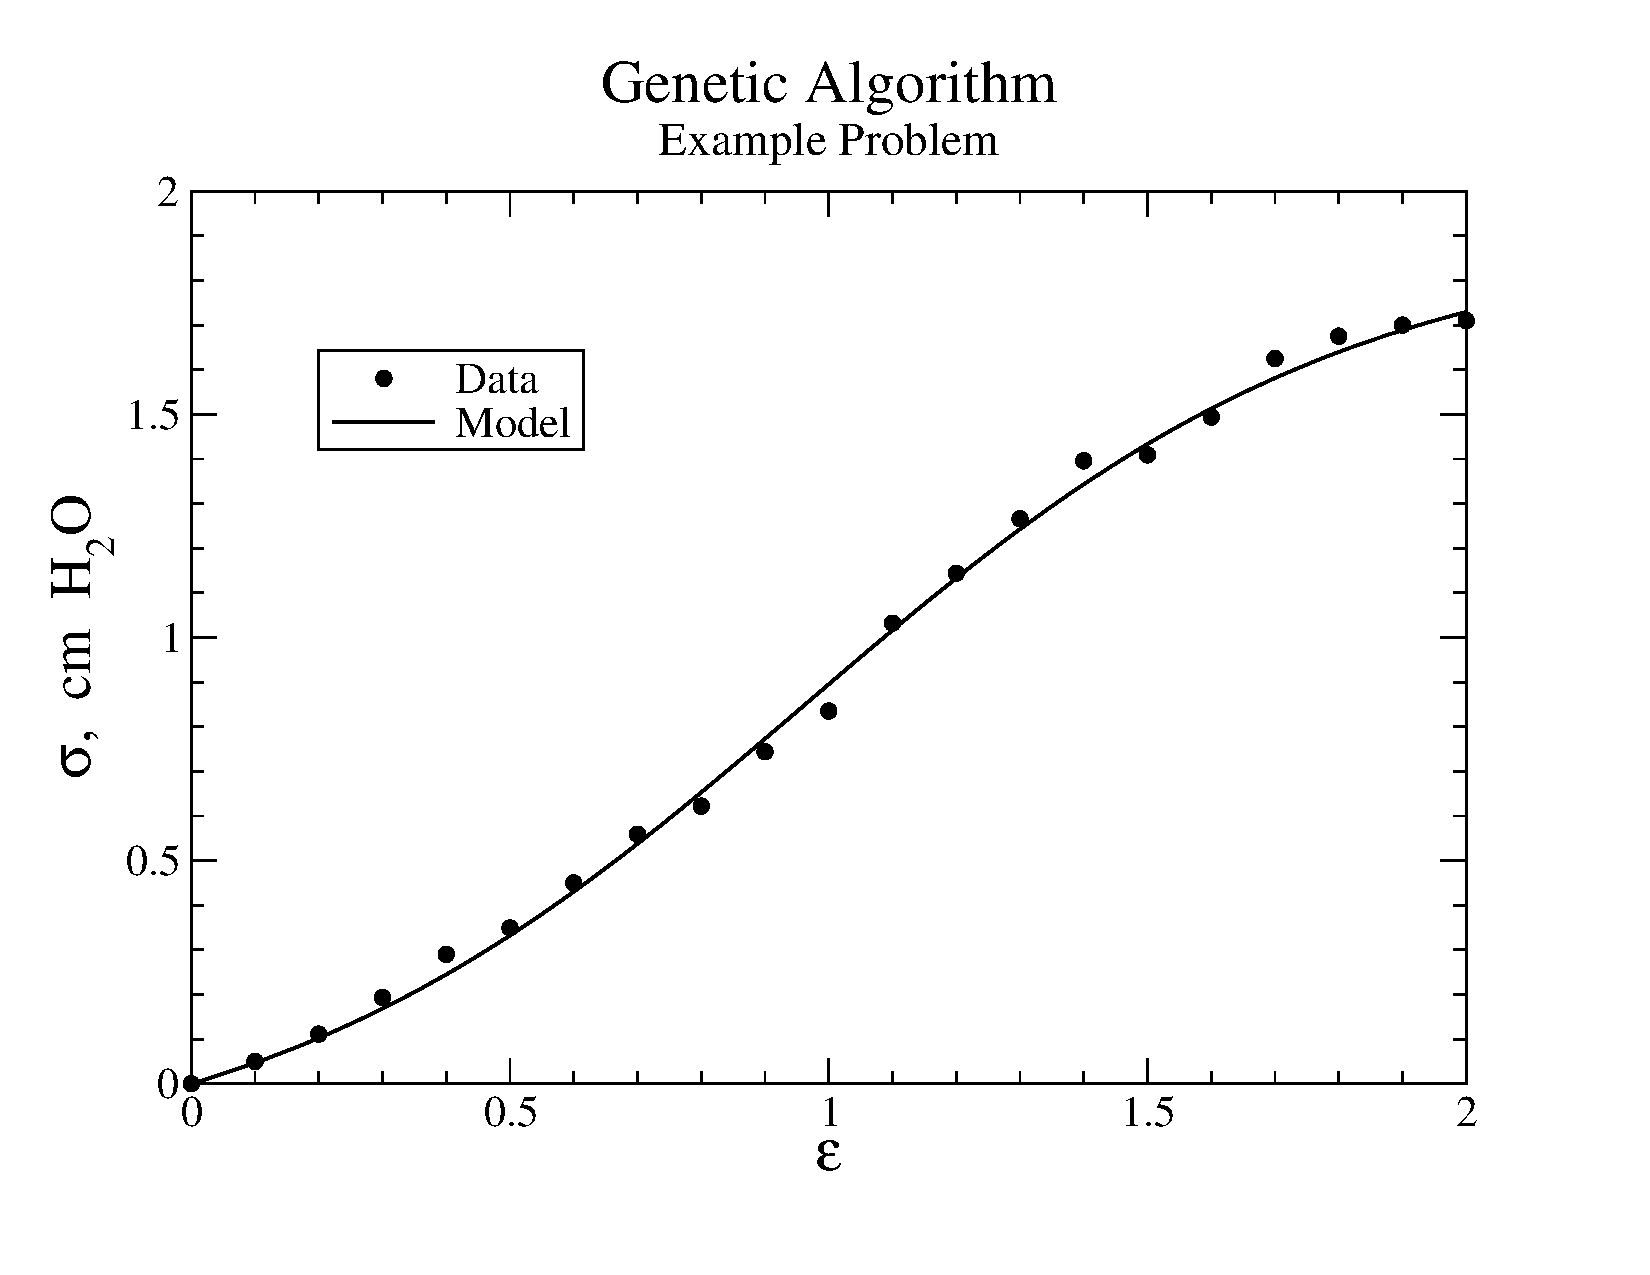
\includegraphics[angle=-90,width=8cm]{gaExample.pdf}
%   \caption{...}
%   \label{...}
%\end{figure}
%
% Double column figure
%\begin{figure*}
%   {\par\centering
%   \resizebox*{1.0\textwidth}{.25\textheight}
%   {\includegraphics[angle=-90]{<figure.eps>}}
%   \par}
%   \caption{\label{<figureLabel>}%
%   }
%\end{figure*}
%
% Tables are the same. A one column table has the structure
%\begin{table}
%  ...
%\end{table}
%
% while a two-column table is created with
%\begin{table*}
%  ...
%\end{table*}
%
%
% Set up babel for typesetting bibliographies.
\usepackage[english]{babel}  %language selection
\selectlanguage{english}
% Languages supported by babel include:
%   american, austrian, brazil, catalan, croatian, czech, danish, dutch,
%   english, esperanto, finnish, french, galician, german, italian, magyar,
%   norsk, nynorsk, polish, portuges, romanian, russian, slovak, slovene,
%   spanish, swedish, turkish.
%
% Select the default text font which is used, for example,
% in the typesetting of the front matter of a paper
% and in the typesetting text in formulae, e.g., sin.
% The Monotype Baskerville fonts are sold separately at: http://www.fonts.com.
%\renewcommand{\rmdefault}{cmr}        % computer modern roman
%\renewcommand{\rmdefault}{txr}        % TX fonts
%\renewcommand{\rmdefault}{ptm}        % Adobe times roman
%\renewcommand{\rmdefault}{mbv}        % Baskerville with inline numbers
\renewcommand{\rmdefault}{mbvj}        % Baskerville with old-style numbers
%
% If AMS-LaTeX macros are to used, load them before mtpro.
% MTPro will replace the AMS fonts, but not its macros.
\usepackage{amsmath, amsthm}
%
% Load MathTime Professional II fonts - commercial fonts
% For sales and other information visit www.pctex.com.
% The following math fonts are created:
%   \mathrm   \mathit    \mathsf   \mathtt
%   \mathbf   \mathbold  \mbf      \mathbb
%   \mathcal  \mathbcal  \mathscr  \mathbscr  \mathfrak
%\usepackage[subscriptcorrection,slantedGreek,boldalphabet,mtpccal,mtpscr,mtpfrak,mtphrb,zswash,nofontinfo]{mtpro2}
\usepackage[subscriptcorrection,slantedGreek,mtpccal,mtpscr,mtpfrak,mtphrb,zswash,nofontinfo]{mtpro2}
%
% Introduce the text fonts.
%
% Define a set of macros for characterizing text fonts.
%   medium fonts   roman     san serif    typewriter
%     upright     \fontrm    \fontss      \fonttt
%     slant       \fontsl    \fontsssl    \fontttsl
%     small cap   \fontsc    \fontsssc    \fontttsc
%     italic      \fontit
%
%   bold fonts     roman     san serif    typewriter
%     upright     \boldrm    \boldss      \boldtt
%     slant       \boldsl    \boldsssl    \boldttsl
%     small cap   \boldsc    \boldsssc    \boldttsc
%     italic      \boldit
%
% Establish the default font encoding scheme to use.
\DeclareFontEncoding{T1}{}{}           % specify text font encoding scheme
\DeclareFontEncoding{TS1}{}{}          % specify text companion font encoding
%
% Normal text fonts.
\DeclareFontFamily{T1}{txr}{\hyphenchar\font=127}
\DeclareFontShape{T1}{txr}{m}{n}{<-> t1xr}{}
\DeclareFontShape{T1}{txr}{m}{sl}{<-> t1xsl}{}
\DeclareFontShape{T1}{txr}{m}{sc}{<-> t1xsc}{}
\DeclareFontShape{T1}{txr}{m}{it}{<-> t1xi}{}
\renewcommand{\normalfont}{\usefont{T1}{txr}{m}{n}}
\newcommand{\fontrm}[1]{\normalfont{#1}}
\newcommand{\fontsl}[1]{\usefont{T1}{txr}{m}{sl}{#1}\normalfont}
\newcommand{\fontsc}[1]{\usefont{T1}{txr}{m}{sc}{#1}\normalfont}
\newcommand{\fontit}[1]{\usefont{T1}{txr}{m}{it}{#1}\normalfont}
%
% Bold text fonts.
\DeclareFontFamily{T1}{txb}{\hyphenchar\font=127}
\DeclareFontShape{T1}{txb}{bx}{n}{<-> t1xb}{}
\DeclareFontShape{T1}{txb}{bx}{sl}{<-> t1xbsl}{}
\DeclareFontShape{T1}{txb}{bx}{sc}{<-> t1xbsc}{}
\DeclareFontShape{T1}{txb}{bx}{it}{<-> t1xbi}{}
\newcommand{\boldrm}[1]{\usefont{T1}{txb}{bx}{n}{#1}\normalfont}
\newcommand{\boldsl}[1]{\usefont{T1}{txb}{bx}{sl}{#1}\normalfont}
\newcommand{\boldsc}[1]{\usefont{T1}{txb}{bx}{sc}{#1}\normalfont}
\newcommand{\boldit}[1]{\usefont{T1}{txb}{bx}{it}{#1}\normalfont}
%
% Normal san serif fonts.
\DeclareFontFamily{T1}{txss}{\hyphenchar\font=127}
\DeclareFontShape{T1}{txss}{m}{n}{<-> s * [0.95] t1xss}{}
\DeclareFontShape{T1}{txss}{m}{sl}{<-> s * [0.95] t1xsssl}{}
\DeclareFontShape{T1}{txss}{m}{sc}{<-> s * [0.95] t1xsssc}{}
\newcommand{\fontss}[1]{\usefont{T1}{txss}{m}{n}{#1}\normalfont}
\newcommand{\fontsssl}[1]{\usefont{T1}{txss}{m}{sl}{#1}\normalfont}
\newcommand{\fontsssc}[1]{\usefont{T1}{txss}{m}{sc}{#1}\normalfont}
%
% Bold san serif fonts.
\DeclareFontFamily{T1}{txssb}{\hyphenchar\font=127}
\DeclareFontShape{T1}{txssb}{bx}{n}{<-> s * [0.95] t1xbss}{}
\DeclareFontShape{T1}{txssb}{bx}{sl}{<-> s * [0.95] t1xbsssl}{}
\DeclareFontShape{T1}{txssb}{bx}{sc}{<-> s * [0.95] t1xbsssc}{}
\newcommand{\boldss}[1]{\usefont{T1}{txssb}{bx}{n}{#1}\normalfont}
\newcommand{\boldsssl}[1]{\usefont{T1}{txssb}{bx}{sl}{#1}\normalfont}
\newcommand{\boldsssc}[1]{\usefont{T1}{txssb}{bx}{sc}{#1}\normalfont}
%
% Normal typewriter fonts.
\DeclareFontFamily{T1}{txtt}{\hyphenchar\font=127}
\DeclareFontShape{T1}{txtt}{m}{n}{<-> t1xtt}{}
\DeclareFontShape{T1}{txtt}{m}{sl}{<-> t1xttsl}{}
\DeclareFontShape{T1}{txtt}{m}{sc}{<-> t1xttsc}{}
\newcommand{\fonttt}[1]{\usefont{T1}{txtt}{m}{n}{#1}\normalfont}
\newcommand{\fontttsl}[1]{\usefont{T1}{txtt}{m}{sl}{#1}\normalfont}
\newcommand{\fontttsc}[1]{\usefont{T1}{txtt}{m}{sc}{#1}\normalfont}
%
% Bold typewriter fonts.
\DeclareFontFamily{T1}{txttb}{\hyphenchar\font=127}
\DeclareFontShape{T1}{txttb}{bx}{n}{<-> t1xbtt}{}
\DeclareFontShape{T1}{txttb}{bx}{sl}{<-> t1xbttsl}{}
\DeclareFontShape{T1}{txttb}{bx}{sc}{<-> t1xbttsc}{}
\newcommand{\boldtt}[1]{\usefont{T1}{txttb}{bx}{n}{#1}\normalfont}
\newcommand{\boldttsl}[1]{\usefont{T1}{txttb}{bx}{sl}{#1}\normalfont}
\newcommand{\boldttsc}[1]{\usefont{T1}{txttb}{bx}{sc}{#1}\normalfont}
%
\usepackage{xspace} % provides appropriate spacing
% Redefine the standard text font selecting macros.
\renewcommand{\textrm}[1]{\fontrm{#1}\xspace}
\renewcommand{\textbf}[1]{\boldrm{#1}\xspace}
\renewcommand{\textit}[1]{\fontit{#1}\xspace}
\renewcommand{\textsc}[1]{\fontsc{#1}\xspace}
\renewcommand{\textsf}[1]{\fontss{#1}\xspace}
\renewcommand{\textsl}[1]{\fontsl{#1}\xspace}
\renewcommand{\texttt}[1]{\fonttt{#1}\xspace}
\renewcommand{\textup}[1]{\fontrm{#1}\xspace}
% If xspace provides unwanted spacing, do not use the
% base \font## or \bold## commands instead of \text##.
%
\newcommand{\eg}{e.g.,\xspace}
\newcommand{\ie}{i.e.,\xspace}
\newcommand{\viz}{viz.,\xspace}
\newcommand{\cf}{cf.\@\xspace}
\newcommand{\eq}{Eq.\@\xspace}
\newcommand{\eqs}{Eqs.\@\xspace}
\newcommand{\etc}{etc.\@\xspace}
\newcommand{\fig}{Fig.\@\xspace}
\newcommand{\figs}{Figs.\@\xspace}
\newcommand{\vs}{vs.\@\xspace}
%
% For underlining options
%\usepackage{ulem}
%    \uline{important}   underlined text
%    \uuline{urgent}     double-underlined text
%    \uwave{boat}        wavy underline
%    \sout{wrong}        line drawn through word
%    \xout{removed}      marked over with //////
%
% Define macros for writing tensor equations.
%
% Macro for typesetting numbers in text.
\newcommand{\scalar}[1]%
   {\fontencoding{TS1}\selectfont #1\fontencoding{T1}\selectfont}
%
% Macros for typesetting vectors - italic roman.
\DeclareMathAlphabet{\mathitbb}{U}{mt2hrb}{m}{it}
\newcommand{\vecFld}[1]{\ensuremath{\mathbold{#1}}}
\newcommand{\vecEle}[1]{\ensuremath{\mathit{#1}}}
\newcommand{\vecMtx}[1]{\ensuremath{\mathitbb{#1}}}
%
% Macros for typesetting tensors of second rank - upright roman.
\newcommand{\tenFld}[1]{\ensuremath{\mbf{#1}}}
\newcommand{\tenEle}[1]{\ensuremath{\mathrm{#1}}}
\newcommand{\tenMtx}[1]{\ensuremath{\mathbb{#1}}}
%
% Macros for typesetting tensors of fourth rank - italic san serif.
\DeclareMathAlphabet{\mathsfbb}{U}{mt2bb}{m}{it}
\newcommand{\TenFld}[1]{\ensuremath{\text{\boldsssl{#1}}}}
\newcommand{\TenEle}[1]{\ensuremath{\text{\fontsssl{#1}}}}
\newcommand{\TenMtx}[1]{\ensuremath{\mathsfbb{#1}}}
%
% Macros for typesetting greek symboled fields.
\newcommand{\grkFld}[1]{\ensuremath{\mathbold{#1}}}
\newcommand{\grkEle}[1]{\ensuremath{#1}}
\newcommand{\grkMtx}[1]{\ensuremath{\mathitbb{#1}}}
%
% Macros for creating nice text and script fractions.
%   There is a cleaner way to do this; for example,
%   \newcommand*{\textfrac}[2]{%
%      {\fontfamily{<fontname>1}\selectfont #1}%
%      \textfractionsolidus
%      {\fontfamily{<fontname>0}\selectfont #2}}%
%   See http://www.ctan.org/tex-archive/macros/latex/doc/fntguide.pdf
%   Sec. V.5: Using the feature of expert fonts
%   Here we must use the following hack because Adobe Times Roman and
%   Baskerville expert fonts do not contain the superior <fontname>1
%   and inferior <fontname>0 glyphs in their font tables.
% Do not break these long lines into multiple lines
% Spaces CANNOT be present - they cause unwanted `rubber' spacing
\newcommand{\textfrac}[2]
   {\leavevmode
    \kern.05em\raise.6ex\hbox{\ensuremath{\scriptstyle{#1}}}\kern-.05em\hspace{0em}/\hspace{0em}\kern-.05em\lower.2ex\hbox{\ensuremath{\scriptstyle{#2}}}\kern.05em
   }
\newcommand{\scriptfrac}[2]
   {\leavevmode
    \kern.05em\raise.3ex\hbox{\ensuremath{\scriptscriptstyle{#1}}}\kern-.05em\hspace{0em}\hbox{\ensuremath{\scriptstyle{/}}}\hspace{0em}\kern-.05em\lower.25ex\hbox{\ensuremath{\scriptscriptstyle{#2}}}\kern.05em
   }
%
% Layout and formatting of the document.
%
% Macro used for creating nomenclatures, etc.
\newcommand{\namelistlabel}[1]{\mbox{#1}\hfil}
\newenvironment{namelist}[1]
   {\begin{list}{}%
      {\let\makelabel\namelistlabel%
       \settowidth{\labelwidth}{#1}%
       \setlength{\leftmargin}{1.1\labelwidth}%
       \setlength{\itemsep}{-6pt}%
      }%
   }{\end{list}%
}
%
% page size
\pdfpagewidth 8.5in
\pdfpageheight 11in
% top margin
\setlength\topmargin{-0.25in}
% header properties
\setlength\headheight{0in}
\setlength\headsep{0in}
% printed size on paper
\setlength\textheight{9.5in}
\setlength\textwidth{7in}
% margins for two-sided printing
\setlength\oddsidemargin{0in}
\setlength\evensidemargin{-0.4in}
% paragraph properties
\setlength\parindent{0.25in}
\setlength\parskip{0.05in}
% Column separation
\setlength{\columnsep}{15pt}
\setlength{\columnseprule}{0pt}
% Fill page
\flushbottom
%
%
% don't hyphenate so much - default = 200, max (never hyphenate) = 10,000
\hyphenpenalty=800
%
% two column float page must be 90% full
\renewcommand\dblfloatpagefraction{.90}
% two column top float can cover up to 80% of page
\renewcommand\dbltopfraction{.80}
% float page must be 90% full
\renewcommand\floatpagefraction{.90}
% top float can cover up to 80% of page
\renewcommand\topfraction{.80}
% bottom float can cover up to 80% of page
\renewcommand\bottomfraction{.80}
% at least 10% of a normal page must contain text
\renewcommand\textfraction{.1}
%
% separation between floats and text
\setlength\dbltextfloatsep{9pt plus 5pt minus 3pt }
% separation between two column floats and text
\setlength\textfloatsep{10pt plus 4pt minus 3pt}
%
%
% Additional declarations beyond my standard template.
%
%%%%%%%%%%%%%%%%%%%%%%%%%%%%%%%%%%%%%%%%%%%%%%%%%%
%
%
%
\begin{document}
%
\bibliographystyle{asme}       % numeric bibliography format
%\bibliographystyle{plain}
%
\title{\textsf{BEL}{\normalfont}--Genetic Algorithm\\
       A \textsf{.NET} Computational Package Written in Zonnon\\
       Part II of the Users Guide\\
       \phantom{A}}
%
\author{Alan D.\ Freed\\
\and
\mbox{}\hfill Clifford H.\ Spicer Chair in Engineering\\
\mbox{}\hfill College of Science, Engineering \& Technology\\
\mbox{}\hfill Saginaw Valley State University\\
\mbox{}\hfill 202 Pioneer Hall, 7400 Bay Road\\
\mbox{}\hfill University Center, MI 48710\\
\mbox{}\hfill E-Mail: \texttt{adfreed@svsu.edu}\\
}
%
\date{\today}

\maketitle
\normalfont

\begin{figure}
   \centering
   
\includegraphics[width=8cm]{BelLogo.pdf}
\end{figure}

\begin{abstract}
This document describes an application library for the \textsf{BEL} framework.  \textsf{BEL} is a
software library written in \textsf{Zonnon} for the \textsf{.NET} and
\textsf{Mono} frameworks.  The application addressed here is that
of a Genetic Algorithm (GA) developed for the purpose of acquiring
parameter estimates belonging to any user-definable mathematical model
that engineers, scientists, and the like would want to use to
describe experimental data or observations through models.
\end{abstract}


\section{Introduction}
\label{introSection}

\textsf{BEL} is an acronym taken for my research laboratory: The Biological
Engineering Laboratory at Saginaw Valley State University. What \textsf{BEL}
is and what it provides are quite different from what one might expect,
given this affiliation. \textsf{BEL} arose out of the author's desire to
interface with the \textsf{.NET} and \textsf{Mono} Frameworks for the purpose
of writing computational software programs in the \textsf{Zonnon} programming
language \cite{Zonnon09}.

\textsf{Zonnon} is the most recent descendant from the family
tree \textsf{Euler}\slash \textsf{Algol}\slash \textsf{Pascal}\slash
\textsf{Modula}\slash \textsf{Oberon} of programming languages
developed by Profs.\ \textsc{Niklaus Wirth} and \textsc{J\"urg Gutknecht}
from the Computer Systems Institute at ETH Zurich (Eidgen\"ossische
Technische Hochschule, Zentrum, \ie the Swiss Federal Institute of
Technology, Zurich).  \textsf{Zonnon} was created specifically for
\textsf{.NET}, with compiler versions available for both the \textsf{.NET}
and \textsf{Mono} Frameworks. Sponsored by Xamarin, Mono is an open 
source implementation of Microsoft's .NET Framework based on the 
ECMA standards for C\# and the Common Language Runtime.
The \textsf{Zonnon} compiler targets the \textsf{.NET} 
Framework~2.0.

The \textsf{Zonnon} compiler, documentation, example programs, 
and even \textsf{BEL} itself, are free to download
from \texttt{http:\slash\slash www.zonnon.ethz.ch}.
The home page for Microsoft's \textsf{.NET} Framework is at
\texttt{http:\slash\slash www.microsoft.com\slash net}.
\textsf{Mono}'s is at
\texttt{http:\slash\slash www.mono-project.com\slash Main_Page}.

Licensing of the \textsf{BEL} library, both its software and
documentation, is addressed in the \textit{Licensing of the
Software and its Documentation\/} part to this user guide.


\subsection{Version}

This document corresponds to software version 4.2 of \textsf{BEL-GAlg},
\today.  \textsf{Zonnon} targets the \textsf{.NET} Framework~2.


\subsection{Required Libraries}

The only external library that is required to compile \textsf{BEL-GAlg} is 
the one that you created when you built \textsf{BEL}.


\subsection{Known Issues}

None


\subsection{Feedback}

I consider this to be a living document. If there is some aspect that is
wanting, or if you have corrections and/or additions that you believe
would benefit other users of \textsf{BEL-GAlg}, please forward them to
\texttt{adfreed@svsu.edu}.


\section{Overview}

\textsc{Goldberg} \cite{Goldberg89} tells his readers what genetic algorithms
(GAs) are, conceptually, in the opening paragraph of his book:
\begin{quotation}
   ``Genetic algorithms are search algorithms based on the mechanics of natural
   selection and natural genetics. They combine survival of the fittest among
   string structures with a structured yet randomized information exchange to
   form a search algorithm with some of the innovative flair of human search.
   In every generation, a new set of artificial creatures (strings) is created
   using bits and pieces of the fittest of the old; an occasional new part is
   tried for good measure. While randomized, genetic algorithms are no simple
   random walk. They efficiently exploit historical information to speculate
   on new search points with expected improved performance.''
\end{quotation}
GAs have in common a population of individuals, a means to determine the
fitness of each individual within the population, the pairing of individuals
for reproduction according to their fitness, the cross-fertilization of
genetic material from parents to produce offspring, and a random chance of a
mutation occurring in the off-springs' genetic code.  A new generation
replaces the existing one, and the reproduction cycle starts all over again.
This process is repeated to convergence, \ie the attainment of a uniform
population of the most fit creature.

Seven modules (presented from the bottom up) were written to implement a
GA for the purpose of obtaining parameter estimates in functions used to
describe observations or experimental data. Their software interfaces are
presented in App.~\ref{gaAppendix}.

The genetic algorithm that is distributed with \textsf{BEL-GAlg} draws
heavily on the algorithms and Pascal code of \textsc{Goldberg}
\cite{Goldberg89,Goldberg02}.  His books focus on what is called a
simple genetic algorithm (SGA), where the probabilities of mutation
and crossover are fixed over the lifetime of the colony.  This software
implements an adaptive genetic algorithm wherein these probabilities
vary over the solution space \cite[pp.~121-122]{SivanandamDeepa08}.
\textsc{Schmitt} \cite{Schmitt01} has shown that GAs can be derived
from the principle of maximum entropy governing a Markovian process.
It turns out that GAs are a great application to showcase the capabilities
of the \textsf{Zonnon} programming language.

GAs are but one of many optimization techniques that exist.  There is a
theorem in the optimization literature called the \textbf{no free lunch}
theorem.  It states that the overall performance of any optimization
algorithm, when evaluated over the set of all possible optimization
problems, is no different than any other optimization technique.  An
apparent advantage of one
algorithm over another resides strictly with its application and, quite
often, the personal taste of the user.  It has been the author's
experience that GAs work very well for parameter estimations of
non-linear material models.


\section{Statistics}

GAs are designed to maximize a fitness pertinent to a species of
\textsl{creatures}. How one defines `fitness' is left for the user
to specify.  The second moment from sample statistics is used
here as the measure for fitness.  An optimal solution is one that minimizes
the noise between experimental data and the model chosen to fit them.
In terms of statistics, this is equivalent to saying that we want to
minimize a variance describing the difference between model and experiment.
GAs choose objective functions that maximize fitness, so in our application
we will select an objective function that is the reciprocal of such a variance,
\ie one arising from the differences between experimental data and their
predictions from a model of correlation.


\subsection{Nomenclature}

\begin{namelist}{$\qquad$}
   \item[$C$] number of control variables
   \item[$N$] number of observations used in optimization
   \item[$O$] total number of experimental observations
   \item[$P$] number of model parameters to be estimated
   \item[$R$] number of response variables
\end{namelist}

\subsection{Random Variables}

There are considered to be $N$, experimental, data vectors $\vecMtx{X}_n$,
$n = 1,2,\dots,N$, that are aggregated as columns into a matrix $\tenMtx{X}
\! = \, \bigr[\!\bigl[ \vecMtx{X}_1 , \vecMtx{X}_2 , \dots , \vecMtx{X}_N
\bigl]\!\bigr]$ wherein each vector $\vecMtx{X}_n$ has $R$ row elements,
\ie $\vecMtx{X}_n = \tenMtx{X} ( t_n )  = \{ x_{1n} , x_{2n} ,
\dots , x_{Rn} \}^T$ evaluated at an instance $t_n$, where $R$ is the number
of responses or dependent variables that have been measured, and $N$
is the number of experimental measurements made.  From these data, estimates
for $P$ parameters $\grkMtx{\theta} = \{ \theta_1 , \theta_2 , \dots ,
\theta_P \}^T$ that belong to some model $\grkMtx{\upXi}(t,\grkMtx{\theta})$
are to be acquired.  A call to procedure \texttt{Theory} returns an $R \times N$
matrix containing its predictions $\grkMtx{\upXi} (t_n, \grkMtx{\theta} )
\! = \, \bigr[\!\bigl[ \grkMtx{\Xi}_1 (\grkMtx{\theta} ), \grkMtx{\Xi}_2
(\grkMtx{\theta} ), \dots , \grkMtx{\Xi}_N (\grkMtx{\theta} ) \bigl]\!\bigr]$,
wherein each column vector $\grkMtx{\Xi}_n$ has $R$ row elements, \ie
$\grkMtx{\Xi}_n(\grkMtx{\theta} ) = \grkMtx{\upXi} (t_n , \grkMtx{\theta}
) = \{ \xi_{1n} (\grkMtx{\theta} ) , \xi_{2n} (\grkMtx{\theta} ) , \dots ,
\xi_{Rn} (\grkMtx{\theta} ) \}^T$ that have been derived using parameters
$\grkMtx{\theta}$.  In what follows, the  $\grkMtx{\theta}$ dependence
of the model $\grkMtx{\upXi} (t_n , \grkMtx{\theta})$, its solution vectors
$\grkMtx{\Xi}_n (\grkMtx{\theta})$, and their components
$\xi_{rn} (\grkMtx{\theta})$ are not explicitly written out in an
effort to keep the notation more compact.  This dependence
is, however, tacitly understood to exist.


\subsubsection{$R=1$}

We begin our discussion by considering a single response variable, \ie
let $R=1$.  For this condition we introduce a random variable to represent
the residual error between two other random variables: one for the experiment,
the other for a model, \viz
\begin{displaymath}
   \vecMtx{e} = a \bigl( \vecMtx{X} - \vecMtx{\Xi} \bigr) ,
\end{displaymath}
whose components are $\vecMtx{e} = \{ e_1 , e_2 , \dots , e_N \}^T$.
To help one acquire a sense of intuition after running multiple
optimizations, it is instructive to introduce a scaling factor $a$ such that
\begin{displaymath}
   a = \frac{1}{\max_{n=1}^N ( | x_n | ) } ,
\end{displaymath}
which places all experimental data within the unit interval $[-1,1]$.
Ideally, one would want the data $a \vecMtx{X}$ to be uniformly dense
over this interval.  If this is not the case with a particular data set
of interest, it may be beneficial to transform it first, \eg by taking its
logarithm.  Of course, this implies that one would have to introduce this
same transformation scheme into one's coding of procedure \texttt{Theory}
that is being used to model these data.  \textit{Parameter estimation is part
science and part art.}

The expected value for this residual error is
\begin{displaymath}
   \mathrm{E} ( \vecMtx{e} ) = a \mathrm{E} ( \vecMtx{X} ) -
   a \mathrm{E} ( \grkMtx{\Xi} )  ,
\end{displaymath}
where sample statistics are used to establish the expectations
residing on the right-hand side of this equation, \viz
\begin{displaymath}
   \begin{aligned}
      \mathrm{E} ( \vecMtx{X} ) & = \frac{1}{N} \sum_{n=1}^N x_n , \\
      \mathrm{E} ( \grkMtx{\Xi}  ) & =
      \frac{1}{N} \sum_{n=1}^N \xi_n  .
   \end{aligned}
\end{displaymath}
From its definition of $\mathrm{VAR} ( \vecMtx{e} ) = \mathrm{E}
( [ \vecMtx{e} - \mathrm{E} ( \vecMtx{e} ) ]^2 )$,
it follows that the variance of this residual error can be described
in terms of the variances and the covariance of its two, dependent, random
variables; specifically,
\begin{multline*}
   \mbox{} \hspace{-4mm} \mathrm{VAR}( \vecMtx{e} ) \\
   = a^2 \bigl( \mathrm{VAR} ( \vecMtx{X} ) +
   \mathrm{VAR} ( \grkMtx{\Xi} ) - 2 \, \mathrm{COV} ( \vecMtx{X} ,
   \grkMtx{\Xi} ) \bigr) ,
\end{multline*}
where the terms on the right-hand side are given by
\begin{displaymath}
   \begin{aligned}
      \mathrm{VAR} ( \vecMtx{X} ) & = \mathrm{E} ( \vecMtx{X}^2 ) -
      \bigl( \mathrm{E} ( \vecMtx{X} ) \bigr)^2 , \\
      \mathrm{VAR} ( \grkMtx{\Xi} ) & = \mathrm{E} ( \grkMtx{\Xi}^2 ) -
      \bigl( \mathrm{E} ( \grkMtx{\Xi} ) \bigr)^2 , \\
      \mathrm{COV} ( \vecMtx{X} , \grkMtx{\Xi} ) & =
      \mathrm{E} ( \vecMtx{X} \grkMtx{\Xi} ) - \mathrm{E} ( \vecMtx{X} )
      \, \mathrm{E} ( \grkMtx{\Xi} ) .
   \end{aligned}
\end{displaymath}
Sample statistics quantifies the second-order moments, too, viz.
\begin{displaymath}
   \begin{aligned}
      \mathrm{E} ( \vecMtx{X}^2 ) & = \frac{1}{N} \sum_{n=1}^N x_n^2  \\
      \mathrm{E} ( \grkMtx{\Xi}^2 ) & =
      \frac{1}{N} \sum_{n=1}^N \xi_n^2  \\
      \mathrm{E} ( \vecMtx{X} \grkMtx{\Xi} ) & =
      \frac{1}{N} \sum_{n=1}^N x_n \, \xi_n
   \end{aligned}
\end{displaymath}
An admissible objective function $\Phi ( \grkMtx{\theta} )$ that can be
maximized by a GA (or like algorithm) is given by
\begin{displaymath}
   \Phi = \frac{ \max_{n=1}^N x_n^2 }
   { \mathrm{VAR} ( \vecMtx{X} ) +
   \mathrm{VAR} ( \grkMtx{\Xi} ) - 2 \, \mathrm{COV} ( \vecMtx{X} ,
   \grkMtx{\Xi} ) } .
\end{displaymath}
This objective function applies for a single response variable.  It will be
at a maximum whenever its denominator is at a minimum, which will occur
whenever the covariance between model and experiment is at its maximum.

Covariance is neglected in almost all optimization strategies,
but here it plays the central role of the process.
\textit{Effectively, the optimization strategy is to
maximize the covariance between model and experiment.}


\subsubsection{$R=2$}

In this scenario we redefine our random variable $\vecMtx{e}$ as
$\grkMtx{\varepsilon}$ to distinguish the sum of two residual errors
$\grkMtx{\varepsilon}$ from its two distinct errors $\vecMtx{e}_1$
and $\vecMtx{e}_2$ as defined in
\begin{displaymath}
   \grkMtx{\varepsilon} = \tfrac{1}{2}
   \bigl( \vecMtx{e}_1 + \vecMtx{e}_2 \bigr) ,
\end{displaymath}
where, like before,
\begin{displaymath}
      \vecMtx{e}_r = a_r \bigl( \vecMtx{X}_r -
      \grkMtx{\Xi}_r \bigr) , \quad r = 1,2,
\end{displaymath}
with
\begin{displaymath}
   a_r = \frac{1}{\max_{n=1}^N ( | x_{rn} |)} , \quad
   r = 1,2,
\end{displaymath}
such that index $r=1$ designates the first response variable,
and $r=2$ the second.

In this case, the expected value for $\grkMtx{\varepsilon}$ is
\begin{displaymath}
   \mathrm{E} ( \grkMtx{\varepsilon} ) = \tfrac{1}{2} \bigl(
   \mathrm{E} ( \vecMtx{e}_1 ) + \mathrm{E} ( \vecMtx{e}_2 ) \bigr) ,
\end{displaymath}
wherein
\begin{displaymath}
   \mathrm{E} ( \vecMtx{e}_r ) = a_r \bigl( \mathrm{E} ( \vecMtx{X}_r ) -
   \mathrm{E} ( \grkMtx{\Xi}_r ) \bigr) ,
\end{displaymath}
with the expectations on the right-hand side of this formula being
evaluated via sample statistics, just as they were defined in the
previous section.  Likewise, the variance of $\grkMtx{\varepsilon}$
is found to be
\small
\begin{multline*}
   \mbox{} \hspace{-4mm} \mathrm{VAR}( \grkMtx{\varepsilon} ) \\
   = \tfrac{1}{4} \bigl( \mathrm{VAR} ( \vecMtx{e}_1 ) +
   \mathrm{VAR} ( \vecMtx{e}_2 ) + 2 \, \mathrm{COV} ( \vecMtx{e}_1 ,
   \vecMtx{e}_2 ) \bigr) ,
\end{multline*}
\normalsize
where here the contribution from the covariance is \textsl{added\/} to that
of its two variances, instead of being \textsl{subtracted\/} as before.  The
variances on the right-hand side of this formula, on the other hand, are described by
\small
\begin{multline*}
   \mbox{} \hspace{-4mm} \mathrm{VAR}( \vecMtx{e}_r ) \\
   = a_r^2 \bigl( \mathrm{VAR} ( \vecMtx{X}_r ) +
   \mathrm{VAR} ( \grkMtx{\Xi}_r ) - 2 \, \mathrm{COV} ( \vecMtx{X}_r ,
   \grkMtx{\Xi}_r ) \bigr) .
\end{multline*}
\normalsize
These variances and covariance are evaluated with sample statistics
in the same manner as their counterparts were in the prior section.

Whenever the two residual errors $\vecMtx{e}_1$ and $\vecMtx{e}_2$
act independent of one another, then, by definition, their covariance
will be zero, \viz \mbox{$\mathrm{COV}(\vecMtx{e}_1 , \vecMtx{e}_2) = 0$,}
which significantly simplifies one's calculation for the total system
variance in that now
\begin{displaymath}
   \mathrm{VAR}(\grkMtx{\varepsilon}) = \tfrac{1}{4} \bigl( \mathrm{VAR}
   (\vecMtx{e}_1) + \mathrm{VAR} (\vecMtx{e}_2) \bigr) .
\end{displaymath}
This simplifying assumption is adopted in this release of the
\textsf{BEL-GAlg} software.

It is important to emphasize that what is being assumed here
is: The \textsl{residual errors\/} $\vecMtx{e}_1$ and
$\vecMtx{e}_2$ are considered to be independent random variables.
This does not imply that their \textsl{response
variables\/} $\vecMtx{X}_1$ and $\vecMtx{X}_2$ are (or are
not) independent of one another.  That is a separate issue.


\subsubsection{Arbitrary $R$}

In a general setting of $R$ separate response variables, one constructs
an overall residual error as a weighted average over all of the individual
residual errors such that
\begin{displaymath}
   \grkMtx{\varepsilon} = \frac{1}{R} \sum_{r=1}^R \vecMtx{e}_r ,
\end{displaymath}
wherein
\begin{displaymath}
      \vecMtx{e}_r = a_r \bigl( \vecMtx{X}_r - \grkMtx{\Xi}_r \bigr) ,
\end{displaymath}
with normalization
\begin{displaymath}
   a_r = \frac{1}{\max_{n=1}^N ( | x_{rn} |)} .
\end{displaymath}
The expectation of this collective residual error is
\begin{displaymath}
   \mathrm{E} ( \grkMtx{\varepsilon} ) = \frac{1}{R} \sum_{r=1}^R \mathrm{E}
   ( \vecMtx{e}_r ) ,
\end{displaymath}
wherein
\begin{displaymath}
   \mathrm{E} ( \vecMtx{e}_r ) = a_r \bigl( \mathrm{E} ( \vecMtx{X}_r ) -
   \mathrm{E} ( \grkMtx{\Xi}_r ) \bigr) ,
\end{displaymath}
while its variance is considered to be described by
\begin{displaymath}
   \mathrm{VAR} ( \grkMtx{\varepsilon} ) = \frac{1}{R^2} \sum_{r=1}^R
   \mathrm{VAR} ( \vecMtx{e}_r ) ,
\end{displaymath}
wherein
\small
\begin{multline*}
   \mbox{} \hspace{-4mm} \mathrm{VAR}( \vecMtx{e}_r ) \\
   = a_r^2 \bigl( \mathrm{VAR} ( \vecMtx{X}_r ) +
   \mathrm{VAR} ( \grkMtx{\Xi}_r ) - 2 \, \mathrm{COV} ( \vecMtx{X}_r ,
   \grkMtx{\Xi}_r ) \bigr) ,
\end{multline*}
\normalsize
with the individual $r$ statistics being quantified as in the
$R=1$ case, but now for each $r$ in $R$.  With this information in hand,
one can propose an objective function for maximization of the form
\begin{displaymath}
   \Phi = \frac{1}{\mathrm{VAR} ( \grkMtx{\varepsilon} )} ,
\end{displaymath}
and our statistical foundation is in place.
A call to \texttt{BelGAlg.Statistics.Fitness} will return
this value of $\Phi$ for a creature with parameters
$\grkMtx{\theta}$.


\subsection{Coefficient of Determination}

Objective functions are powerful tools in applications,
but they can be difficult to acquire an intuitive feel for `goodness of fit'.
The coefficient of determination is not unique when extended
to non-linear optimization algorithms, and many methods for
computing such an $\mathcal{R}^2$ value have been proposed over the
years.  An adjusted or bias corrected coefficient of determination taken from
multiple regression analysis has been applied here; specifically,
\begin{displaymath}
  \mathcal{R}^2 = 1 - \frac{N-1}{N-P} \,
  \frac{\mathrm{E} (\grkMtx{\varepsilon}^2)}
  {\mathrm{VAR} (\tenMtx{X})} ,
\end{displaymath}
where
\begin{displaymath}
   \mathrm{VAR} (\tenMtx{X}) = \frac{1}{R^2} \sum_{r=1}^R a_r^2
   \mathrm{VAR} (\vecMtx{X}_r) ,
\end{displaymath}
and
\begin{displaymath}
   \mathrm{E} ( \grkMtx{\varepsilon}^2 ) = \frac{1}{R^2} \sum_{r=1}^R
   \mathrm{E} ( \vecMtx{e}_r^2 ) ,
\end{displaymath}
wherein
\begin{displaymath}
   \mathrm{E} ( \vecMtx{e}_r^2 ) = a_r^2 \bigl(
   \mathrm{E} ( \vecMtx{X}_r^2 ) + \mathrm{E} ( \grkMtx{\Xi}_r^2 ) -
   2 \, \mathrm{E} ( \vecMtx{X}_r \grkMtx{\Xi}_r ) \bigr) .
\end{displaymath}
As with the variance of residual error $\mathrm{VAR} ( \grkMtx{\varepsilon} )$,
it is assumed that the squared errors of the residuals $\vecMtx{e}^2_1$,
$\vecMtx{e}^2_2$, $\dots$, $\vecMtx{e}^2_R$ are independent of one another,
too, and therefore there expectations can be summed.  We recall that
$\mathrm{VAR} ( \grkMtx{\varepsilon} ) = \mathrm{E} ( \grkMtx{\varepsilon}^2 ) - (
\mathrm{E} ( \grkMtx{\varepsilon} ))^2$ and $\mathrm{VAR} ( \vecMtx{e}_r ) =
\mathrm{E} ( \vecMtx{e}_r^2 ) - ( \mathrm{E} ( \vecMtx{e}_r ))^2$
$\forall$ $r$, where the supposition is that like terms sum over $R$.
Here $P$ is the dimension of $\grkMtx{\theta}$, \ie the
number of parameters that are fit, $R$ is the number of response
variables being modeled, and $N$ is the number of datum
points being fit against.  Procedure \texttt{RSquared} in
module \texttt{BelGAlg.Statistics} returns this adjusted
$\mathcal{R}^2$ statistic for a given set of parameters
$\grkMtx{\theta}$.  The parameters that maximize the fitness function
$\Phi$ are typically distinct from those that maximize the $\mathcal{R}^2$
statistic, although they are similar.

It bears repeating a phrase that commonly appears whenever an
$\mathcal{R}^2$ statistic is being introduced: ``Correlation
does not imply causation.''  In other words, good correlation
(a high $\mathcal{R}^2$ statistic) must not be used to infer
or suggest the existence of a causal relationship between a
model and data, \ie it does not prove that the model is `correct'.


\subsection{The Software}

Module \texttt{BelGAlg.Statistics} exports four immutable constants:
the number of data sets being fit against $N$ as \texttt{dimN},
the number of response or independent variables $R$ in the
experiment\slash model as \texttt{dimR}, the number of control
or dependent variables \texttt{dimC} (which must equal \texttt{dimR}
whenever the data are to be decimated), and the number
of parameters allowed to vary $P$ that appear within a model
as \texttt{dimP}.  It also exports
two probabilistic functions that are used throughout the
GA modules: a biased coin flip via \texttt{FlipHeads}, and the
return of a \texttt{RandomIntergerBetween} two distinct integers.

\texttt{Statistics} also exports a procedure type.  Instances of
\texttt{Model} can be submitted to the GA for parameter optimization.
They get passed to either procedure \texttt{Optimize} or
\texttt{Easy\-Optimize} in module \texttt{BelGAlg.GeneticAlgorithm}.
Type \texttt{Model} requires two arguments.  The first is a
\textsf{Bel.Types.RealVector} of length $P$ that contains the parameters
to be estimated. The second is a \textsf{Bel.Types.RealMatrix}
with $C$ rows (the number of control variables) and $O$ columns
(the total number of experimental observations).  A call to a
\texttt{Model} implementation will return a \textsf{Bel.Types.RealMatrix}
in $R$ rows, which is the number of response variables,
spanning over the $O$ columns.  It contains the predicted response of
the model when subjected to the supplied control variables for the
given set of model parameters.

Procedure \texttt{Configure} allows the user to supply experimental data,
and a numerical model whose parameters one hopes to estimate. This procedure
has five arguments, the first two of which contain experimental
data.  The first is a $C \times O$ matrix that holds the control variables
to be forwarded to the user-supplied model.  The second is a
$R \times O$ matrix that contains the experimental
output variables, the latter of which the optimizer will attempt to
replicate with the model by systematically adjusting its parameters.

The third argument of \texttt{Configure} indicates how many of the
data points are to be used for optimization.  Optimization is an
expensive process, and it is often useful to decimate larger data
sets into smaller more manageable ones.  A decimation scheme similar
to that of \textsc{Doehring} \textit{et~al.} \cite{Doehringetal04} has
been implemented into \texttt{Configure}, where the input\slash output
curves are segmented into intervals of like arc length.  \textbf{Note}:
Decimation requires the input and output matrices to
have the same dimensions.

The fourth argument supplies the numerical model to the optimizer,
while the fifth selects which model parameters are
to be allowed to vary.  It may be that you know a parameter
\textsl{a~priori\/} so there is no need to allow
the optimizer to seek its value.

Procedure \texttt{DataFitAgainst} returns the decimated experimental
data set used for parameter estimation.  The two arguments are
matrices.  The first has dimension $C \times N$ while the second
has dimension $R \times N$, where $C$ is the number of control
variables, $R$ is the number of response variables, and $N$ is
the actual number of experimental data points used during an optimization,
\ie $N \leq O$.  The first argument contains the experimental inputs.
The second argument contains the experimental outputs.
They are subsets of the first two
arguments supplied to \texttt{Configure}.  This information
may be useful to the user who may want them, \eg to make
graphs of a model's capability to correlate these data.

For these data that are to be fit against, procedure
\texttt{Theory} returns their corresponding theoretical predictions using
the model assigned previously to the GA via procedure \texttt{Configure}.
\texttt{Theory} requires that the caller send the set of
model parameters that are to be used by the theory to
provide its predictions, which are returned as a $R \times N$ matrix.


\section{Genes}

A gene is an information bit in a memory bank that belongs to the overall
cache of biological memory that resides within a living organism, often
referred to in the GA literature as a \textit{creature}.

Module \texttt{BelGAlg.Genes} exports type \texttt{Gene}, which
implements definitions \texttt{Bel.Entity} and \texttt{Bel.Typeset}.

The implementation of \texttt{Initialize} applies even-odds probability
to assign a random value for its allele (the expression of that gene).
Allele are randomly assigned in the beginning, \ie during the procreation, which is
where the first colony of individuals originates from,
and whenever an individual immigrates into the colony. In later colonies,
the allele are assigned through chromosome splitting (occurs with high
probability) with the possibility of an additional gene mutation (occurs
with small probability), both of which take place at the time of reproduction.

Method \texttt{Clone} produces a duplicate of its genetic
material that from a biological perspective makes it the appropriate
terminology to use to describe its action.  In computer science, however,
a clone would have the same type, but it would be an empty shell of
the original, minus any substantive data, which is how a
\texttt{Bel.Object.Clone} is typically implemented.  (\texttt{Gene}
does not implement the \texttt{Bel.Object} interface.)

\texttt{Parse} and \texttt{Print} are used to assign and extract the
allele of a gene after its initial creation. This is done with strings.
A biallelic gene is implemented which has two expressive states: dominant
and recessive. Dominant genes are expressed with a 1, while recessive genes
are expressed with a 0.\footnote{%
   In versions 1.2.1 and earlier, a triallelic gene was also implemented.
   It had three expressive states: dominant, dominant\slash recessive and
   recessive, where a dominant gene was expressed with a 1, a dominant\slash
   recessive gene was expressed with a \%, and a recessive gene was
   expressed with a 0.  Experimentation with this option found that it
   brought little to no added value to the overall optimization process,
   so it was removed with the release of version 2.0 of the software.
}

Methods \texttt{Pop} and \texttt{Put} are for internal use in that
they are called by the operator overloading assignment; specifically:
\newline\boldtt{operator}\fonttt{ ":=" (}\boldtt{var}
\fonttt{ l\;:\;Gene; r\;:\;Gene);} \\
\boldtt{begin} \\
\indent\fonttt{l.Put(r.Pop())} \\
\boldtt{end}\fonttt{ ":=";}\newline
This technique allows one to make deep copies of an object via assignment
without utilizing the assignment operator $:=$ in its implementation.

Method \texttt{Mutate} performs a random mutation on a gene,
switching its value at some specified probability for mutation. If a gene is
mutated, it increments a counter that is used to keep track of the number
of mutations that have occurred for output into the final report, \cf
App.~\ref{GaAppendix}.

Method \texttt{Equals} tests two genes to determine if they are
equivalent.  It is called by the overloaded operators ``\texttt{=}'' and
``\texttt{\#}''.


\subsection{Probability of Mutation}

In simple genetic algorithms (SGA), like the one developed in the book
of \textsc{Goldberg} \cite{Goldberg89}, the probability of a mutation
occurring is held fixed over the life of a colony of creatures.  An
adaptive genetic algorithm \cite[pg.~122]{SivanandamDeepa08} is employed
in \textsf{Bel-GAlg}.  After a generation has been fully populated and
the fitness of all creatures in that generation are known, an adaptive
probability of mutation $P_m$ is then assigned to each creature according
to the formula (which has a typo in \cite{SivanandamDeepa08})
\begin{displaymath}
   P_m = \begin{cases}
   P^m_{\text{max}} - \frac{(P^m_{\text{max}} - P^m_{\text{min}})
   (f - f_{\text{avg}})}{f_{\text{max}} - f_{\text{avg}}} &
   f \geq f_{\text{avg}} , \\
   P^m_{\text{max}} & f < f_{\text{avg}} ,
   \end{cases}
\end{displaymath}
where $P^m_{\text{max}}$ and $P^m_{\text{min}}$ are the maximum and
minimum probabilities for mutation, which are exported from module
\texttt{BelGAlg.Creatures} through the pair of constants 
\texttt{maxProbabilityOfMutation}
and \texttt{minProbabilityOfMutation}, where they are assigned values of
$0.1$ and $0.001$, respectively.  The fitness of an individual creature is
denoted as $f$, while $f_{\text{avg}}$ and $f_{\text{max}}$ correspond
to the average fitness of that generation's population and the
fitness of its \textsl{elite\/} creature.  This formula is akin to
the annealing protocol derived by \textsc{Schmitt} \cite{Schmitt04}.

At the time of reproduction, the probability of mutation applied to
an offspring is the average of the probabilities of mutation belonging
to its parents.


\section{Chromosomes}

A chromosome is a bank of memory comprised of a string of genes that
is part of the overall cache of biological memory that resides within
a living organism.  In genetic algorithms, a creature's chromosome is
a register or memory cache for a parameter whose value is being sought via the GA.

In this implementation of a GA, each chromosome is paired with a single
model parameter that is being sought through optimization. If a model
has five unknown parameters that are to be estimated, for example, then
its implementation in \textsf{BEL-GAlg} will result in five unique chromosomes.
In this respect, \textsf{BEL-GAlg} differs from \fontsc{Goldberg}'s SGA
\cite{Goldberg89}.  His SGA has just one chromosome, whose genotypes
for all of the parameters are spliced into a long single strand of genes.

Module \texttt{BelGAlg.Chromosomes} exports type \texttt{Chromosome},
which is an implementation of the \texttt{[]}, \texttt{Bel.Entity},
and \texttt{Bel.Typeset} definitions.  \texttt{Chromosome}
is a wrapper for the other exported type: \texttt{Haploid}, which is
an \textbf{array * of} \texttt{BelGAlg.Genes.Gene}.\footnote{%
   In versions 1.2.1 and earlier, a diploid chromosome, which is a
   string of triallelic genes, was also implemented.  Experimentation
   with this option found that it too brought little additional value to
   the overall optimization process, so it was removed with the release
   of version 2.0 of the software.
}
Type \texttt{Chromosome} exports seven methods, in addition to the four
that are required by the three definitions being implemented.

Method \texttt{Clone} returns an exact duplicate of itself, \ie a
deep copy.  \texttt{Chromosome} assignment via $:=$ yields a shallow
copy.   To get a deep copy one must call \texttt{Clone}. 
(\texttt{Chromosome} does not implement the \texttt{Bel.Object} 
interface.)

Method \texttt{Create} receives the lower and upper boundaries that
establish the regions of search associated with each parameter, each
being assigned to their own chromosome.  Also supplied is
the number of significant figures in accuracy that one would hope to
have in the final result (the author used 4 in the following example).
These three factors establish the number of genes required by each
chromosome, whose collective sum (over all chromosomes) is exported
through method \texttt{Length}.

Method \texttt{Equals} checks to see if the strings of gene expression
between the two chromosomes are the same.  \texttt{Equals} is called by
the overloaded operators ``\texttt{=}'' and ``\texttt{\#}''.

Method \texttt{Mutate} forwards its call to all genes within the
chromosome string, where the actual mutations take place.

\texttt{Encode} and \texttt{Decode} are analogs to \texttt{Parse} and
\texttt{Print}, except they import and export the \textsl{pheno\-type\/}
(\ie the model parameter) held by the chromosome; whereas, \texttt{Parse}
and \texttt{Print} import and export the \textsl{genotype}
(the values of their allele). \texttt{Encode}
and \texttt{Decode} provide the mapping functions that bridge a model
(whose parameters are to be estimated) with the GA that will estimate them.

Gene expression is \textsc{Gray} encoded in our GA \cite{Michalewicz96}.
\textsc{Gray} numbers are a binary-like representation whose neighboring
values differ by one bit only, which is not true of binary numbers.
\textsc{Gray} code is mapped into binary code. Binary code is mapped
into integers. And integers are then converted into their corresponding
real phenotype in \texttt{Decode}. \texttt{Encode} runs these maps in reverse.

E.g., a \texttt{BelGAlg.Chromosomes.Chromosome} could have a genotype that
looks like
\begin{displaymath}
   \begin{array}{cccccccc}
       1 & 0 & 0 & 1 & 0 & 1 & 1 & 1
   \end{array}
\end{displaymath}
that, in this case, is a string of eight biallelic genes.  The \texttt{Get}
and \texttt{Set} procedures (called by its indexer via the \texttt{[]}
interface) can access the individual genes in a chromosome, and accept
indexes between 0 and $\mathtt{Length} - 1$.

A chromosome has two types of riders that position differently.
An `index' rider points directly to a gene, and is used for mutation.
Its value resides within the interval $[0, \mathtt{Length} - 1]$.
A `locus' rider points in between two genes, and is used for crossover
(chromosome splitting). Its value belongs to the interval
$[1, \mathtt{Length}-1]$.  The overloaded indexer for a
\textsf{BEL-GAlg} chromosome associates with a chromosome's
`index' rider.

Module \texttt{BelGAlg.Chromosomes} also exports the procedure
\texttt{Crossover}, which is called by \mbox{higher}-level modules to
mate two individuals and return their offspring. This is where
crossover (the splitting and splicing of chromosomes at reproduction)
actually occurs. The first argument establishes the probability for
crossover to occur. The second and third arguments provide the happy
parents. The fourth argument is a counter that gets incremented if
crossover takes place; it is a statistic provided in the final report.
The final pair of arguments are the offspring of this mating,
which will be clones of their parents if no crossover takes place.

\texttt{Crossover} implements a one-point crossover procedure
\cite{SivanandamDeepa08}.  As an example, consider two parents whose
chromosomes are of length six.  From a call to a random number generator
it is determined that a splice is to take place between the second
and third genes, \eg and therefore
\begin{displaymath}
    \begin{array}{ccccc}
        1 & 0 \; | \; 1 & 1 & 0 & 0 \\
        0 & 1 \; | \; 0 & 1 & 0 & 1
    \end{array}
    \; \longrightarrow \;
    \begin{array}{ccccc}
        1 & 0 \; | \; 0 & 1 & 0 & 1 \\
        0 & 1 \; | \; 1 & 1 & 0 & 0
    \end{array} ,
\end{displaymath}
where the parents on the left produce the children on the right in
this example.

Schemata are the building blocks of genetic algorithms; they are what make
them work \cite{Goldberg89,Goldberg02}.  A schema can be any string of genes
that is shorter than a chromosome; it is a subset to a chromosome.  In a
genetic algorithm, high-performance, low-order schemata receive exponentially
increasing numbers of trials in successive generations, which leads to the
fundamental theorem of genetic algorithms \cite{Goldberg89,SivanandamDeepa08}.
This is why they outperform other stochastic methods, like Monti Carlo
techniques.  In schemata, some of the genes take
on fixed expressions, while others are allowed to have any expression,
and are denoted with a $\star$.  For example, a schema might
look like $\begin{array}{ccc} 1 & \star & 0 \end{array}$ of which
instances $\begin{array}{ccc} 1 & 0 & 0 \end{array}$ and
$\begin{array}{ccc} 1 & 1 & 0 \end{array}$ would both belong.  In this
example, the schema has dimension three.  In the example that
follows, schemata up to dimension 6 were used.


\subsection{Probability of Crossover}

In SGAs, the probability of a crossover occurring within any given
chromosome during reproduction is held fixed over the life of a
colony of creatures.  An adaptive genetic algorithm is employed in
\textsf{Bel-GAlg} with the probability of crossover varying along
the solution path.  After a generation has been fully populated
and the fitness of all creatures in that generation are known,
an adaptive probability for crossover $P_c$ for every chromosome
belonging to an individual creature is then assigned according
to the formula
\begin{displaymath}
   \mbox{}\hspace{-2mm}
   P_c = \frac{1}{P} \begin{cases}
   P^c_{\text{max}} - \frac{(P^c_{\text{max}} - P^c_{\text{min}})
   (f - f_{\text{avg}})}{f_{\text{max}} - f_{\text{avg}}} &
   f \geq f_{\text{avg}} , \\
   P^c_{\text{max}} & f < f_{\text{avg}} ,
   \end{cases}
\end{displaymath}
where $P^c_{\text{max}}$ and $P^c_{\text{min}}$ are the maximum and
minimum probabilities for crossover occurring within a creature,
which are exported from the module \texttt{BelGAlg.Creatures}
through the constants \texttt{maxProbabilityOfCrossover}
and \texttt{minProbabilityOfCrossover}. There they are assigned
values of $0.9$ and $0.6$, respectively.  Here $P$ designates the
number of chromosomes (or material parameters in a model) that
belong to a creature.  The fitness of the creature is
denoted as $f$, while $f_{\text{avg}}$ and $f_{\text{max}}$ correspond
to the average fitness of that generation's population and the
fitness of its \textsl{elite\/} creature.  This formula is akin to
an annealing protocol, a consequence derived by \textsc{Schmitt}
\cite{Schmitt04} to ensure convergence.

At the time of reproduction, the probability of crossover applied to
an offspring is the average of the probabilities of crossover belonging
to its parents.


\section{Genomes}

A genome is the whole cache of biological memory.  It contains the
entire evolutionary history of a living organism.  In a GA, it contains
the genetic imprint of a creature.

This GA differs from SGA by including the concept of a genome, taken here
to be the collection of all chromosomes belonging to an individual.
Recall that each model parameter associates with its own chromosome.
Therefore, there is a one-to-one correlation between the array of numbers
that are a model's parameters and the array of chromosomes that comprise
its genome. Different models will have different genome; they are akin to
being different species. In contrast, the human has 23 diploid chromosomes.
Each is comprised of two gene strings.  One string is taken from each parent.

Module \texttt{BelGAlg.Genomes} exports the ancillary data type \texttt{Genotype},
which is an \textbf{array * of} \texttt{BelGAlg.Chormosomes.Chromosome} for
which the predominant type \texttt{Genome} is a wrapper.  Type \texttt{Genome}
implements two definitions; they are: \texttt{[]} and \texttt{Bel.Entity}.

Via \texttt{Genome}'s implementation of the \textsf{Zonnon} indexer
\texttt{[]}, access is gained to the various chromosomes in a genome,
with admissible values belonging to the interval $[0, \mathtt{Strands}-1]$,
where method \texttt{Strands} returns the number of chromosomes in the genome,
\ie the number of parameters to be estimated.

Method \texttt{Clone} returns an exact duplicate of itself.  Assignment
$:=$ returns a shallow copy of a \texttt{Genome}.  (\texttt{Genome} does
not implement the \texttt{Bel.Object} interface.)

Method \texttt{Equals} compares two genome, and is called by the
overloaded operators ``\texttt{=}'' and ``\texttt{\#}''. It tests for
equality of gene expression.

Methods \texttt{Mutate}, \texttt{Encode} and \texttt{Decode} all forward
their requests down to its chromosomes, where the appropriate actions are
taken.

Module \texttt{BelGAlg.Genomes} exports two procedures; they are
\texttt{Crossover} and \texttt{Similarity}. \texttt{Crossover}
redirects the request to its underlying individual chromosomes
for action.  \texttt{Similarity} compares two genome, returning
the fraction that are the same, \ie the number of genes where
both genome have the same allele, divided by the number of genes
in the genome.  This value is reported on for the elite creature
of each generation in the final report, \cf App.~\ref{GaAppendix}.
Because clones are not permitted in this GA (they are in some),
its value will always be below 1.0. As the solution converges,
this quantity ought to become close to~1.


\section{Creatures}

We now move up to the level of a physical being, an entity, or an organism.
The module \texttt{BelGAlg.Creatures} exports type \texttt{Lineage},
which keeps track of an individual's assets. This type makes
available a creature's \texttt{birthID}, which is akin to a
social security number; its \texttt{fitness}, which determines its
chances for mating; its parameters, which establish its genetics;
the similarity of its parent's genome \texttt{parentSimilarity},
which is their fraction of allele with the same gene expression; its
\texttt{probabilityOfMutation}, which adapts dynamically (\ie it
anneals) with the solution; and its \texttt{probabilityOfCrossover},
which also adapts with the evolving solution.  \texttt{Lineage}
implements the \texttt{Bel.Object} interface because \textsf{BelGAlg}
uses a \texttt{Bel.List} to store the lineage of all creatures
belonging to a colony so that a report (\cf App.~\ref{GaAppendix})
can be written.

The main type exported by this module is a \texttt{Creature},
which implements the \texttt{Bel.Entity} interface.  Method
\texttt{Clone} returns a deep copy of itself; whereas, assignment $:=$
returns a shallow copy.  Method \texttt{Create} should be called
immediately after a creature is created via the \textbf{new} command.
Two arguments are passed with this call. The first, \texttt{fixedParameters},
is an array of those model parameters that the user chooses to fix, \ie the
optimizer will not vary these.  If all of the parameters are to vary, then
\texttt{fixedParameters} is \textbf{nil}. The second argument,
 \texttt{varyParameters},
is a boolean array designating which variables are to be held fixed
and which are allowed to vary, as they are passed to a model of
type \texttt{BelGAlg.Statistics.Model}. Say, \eg that your model
has 5 parameters, the second and fifth of which you can get reliably
from a graphical method.  In this case, \texttt{varyParameters} would be
a boolean array of length 5 with values $\{ T, F, T, T, F \}^T$.

Each individual has a unique phenotype that associates with a unique
set of model parameters that are stored in its \texttt{lineage} as
\texttt{parameters}.  This array of the model's parameters contains
both those that are fixed and those that have been allowed to vary.

Two individuals can be discerned as being clones of one another via
the method \texttt{Equals}, which is called by the overloaded operators
``\texttt{=}'' and ``\texttt{\#}''.

An individual's genome can be retrieved with method \texttt{Get}.

Probabilities for mutation and crossover, as they pertain to a
specific creature, are assigned by the method \texttt{AssignProbabilities},
where the first argument specifies the maximum fitness of the population
and the second argument specifies the average or mean fitness of the
population.

An individual can come into being via three different routes.
\texttt{Procreate} is used to create the first colony of individuals,
and to create immigrants from outside the colony.  \texttt{Procreate}
introduces a Monti Carlo event into the optimization process.
It requires arguments that specify the lower and upper bounds
defining the interval that each parameter is allowed to vary over,
and the number of significant figures in accuracy hoped for in the
parameters' final values.

The second way an individual can be created is by an \texttt{Alien}
migrating into the population. An alien individual has the same arguments
that a procreated individual does, plus it specifies what its phenotype is
(\ie its model parameters); whereas, a procreated individual has its
phenotype assigned by chance.  An alien can be thought of as `seeding'
a population with an individual thought to have good fitness.  In a certain
sense, \textsf{BelGAlg} seeds each new generation with an alien---the
most fit or elite creature from the previous generation.

The third and final way to create an individual is to \texttt{Conceive}
it through the mating of two distinct individuals, \ie its parents,
which are the first two arguments passed in \texttt{Conceive}.  This
method produces a new \texttt{Creature}, \viz their child.  It also
updates the counters \texttt{numberOfMutations} and
\texttt{numberOfCrossovers}, whose tallies are statistics tabulated
in the report (\cf App.~\ref{GaAppendix}).  A call to \texttt{Conceive}
may also introduce an immigrant, at a probability of once per generation,
as an aid to maintaining a diverse genetic pool within a population
and to help ensure convergence \cite{YaoSethares94}.
Clones are not permitted within a population.  In some GAs
\cite{Schmitt01}, convergence occurs when the whole population consists
of clones of a single creature.  That philosophy is not adopted here.


\section{Colonies}

The highest level in the hierarchy of our GA (there are five levels)
is a population of creatures that makes up the colony at a moment in
its history.  Pairs of creatures from an existing colony are selected
for mating through tournament play, whose offspring will comprise the
next generation for the colony.  The contestants for tournament play
are selected at random from the existing population of individuals,
with the most-fit contestant from each tournament of play being selected
to mate.  The number of contestants $s$ in tournament play is set at
2\% of the population size, but must be at least 3 in count.

Some GAs allow their population size to vary from one generation to the
next. However, the colony size $n$ of this GA is held fixed over all the
generations, assigned internally according to the formula~\cite{Goldberg02}
\begin{displaymath}
   n = \bigl\lceil \chi^k ( k \ln \chi + \ln \ell ) \bigr\rceil,
\end{displaymath}
where $\chi$ is the cardinality of the gene alphabet being used (\eg 2 for
haploid, 3 for diploid, \etc), $k$ is the bounding dimension for which all
schemata up to that length are to be successfully sampled, recombined,
and re-sampled, while $\ell$ is the number of genes in the genome.  The
user affects this value through his\slash her choices for the variables
\texttt{dimensionOfSchemata} and \texttt{numberOfSignificantFigures},
the former of which is assigned to $k$, and the latter through its influence
on the number of genes $\ell$ required by the encoder\slash decoder.

A truly remarkable result is that the number of generations needed for convergence
$t_c$ can be estimated \textit{a~priori\/} via the formula~\cite{Goldberg02}
\begin{displaymath}
   t_c = \bigl\lceil \sqrt{\ell} \: \ln n / \ln s \bigr\rceil ,
\end{displaymath}
where $\ell$ is the number of genes in the genome, $n$ is the number of
creatures that constitutes a population, and $s$ is the number of
contestants in tournament play.  After $t_c$ generations have been
created, a message will be displayed in the terminal window providing
the user with certain information to help them determine if more
generations are needed, or if the solution is acceptable.  Although
theory specifies $t_c$, in practice this predetermined number of
generations may not be enough to achieve convergence.

Module \texttt{BelGAlg.Colonies} exports two types. The predominant type,
\texttt{Colony}, places a wrapper around \texttt{Inhabitants}, which is
an \textbf{array * of} \texttt{BelGAlg.Creatures.Creature}.
\texttt{Colony} implements the \texttt{Bel.Entity} interface.

To \texttt{Create} a \texttt{Colony} requires a whole slew of arguments.
The first five are the same as those required by \texttt{Statistics.Configure}.
After that there are: an array (set to \textbf{nil} if of zero length)
containing parameters whose values the optimizer cannot adjust, a set of
alien parameters introduced to seed the optimizer, lower and upper bounds to
establish search intervals over which an optimal set of parameters is thought to be found.
(The last three of these arrays pertain to only those parameters whose values
the optimizer is allowed to adjust.)  This is followed by the dimension
of schemata that are to be captured, and the number of significant figures
in accuracy that are desired in the solution.

Method \texttt{Propagate} advances the colony to its next generation.

Method \texttt{Parameters} returns the phenotype from the elite individual
in the colony for the current generation.

The remaining methods are used to write a report to file. They provide
a condensed version for the history of a colony, along with a number
of useful statistics, and the optimum parameters found in that search.
The number of individuals that lie within intervals of $\pm$ a precision
loss of half the number of significant figures, which is documented
in the report, provides a sense of how well a particular optimization
run performed.  As a rule of thumb, at least 10\%\ of the
total population size ought to lie within this range.
Smaller values suggest that one needs to refine one's search strategy.
\texttt{ReportHeader} is to be called before the first generation is
brought into existence. \texttt{ReportBody} can be called after the
arrival of any new generation. And \texttt{ReportFooter} is to be
called after the final generation has been born and reported on.
Appendix \ref{GaAppendix} contains an example of such a report.
Method \texttt{CheckOnTheState} reports the current state of the
optimizer to a terminal window to allow the user to either terminate
or continue with an optimization.

\section{Genetic Algorithm Driver}

Module \texttt{BelGAlg.GeneticAlgorithm} exports two funtions:
\texttt{Optimize} and \texttt{EasyOptimize}. They are the drivers of
\textsf{BelGAlg}.  They return the optimal set of parameters found 
by the genetic algorithm. There are twelve arguments in \texttt{Optimize}
that must be sent to this driver, and six for \texttt{EasyOptimize}.
All twelve are discussed in some detail, as this is the interface
that most programmers will use in order to obtain an optimal set
of estimated parameters.  \texttt{EasyOptimize} calls on a subset
of these twelve, using defaults for the other six.  If the defaults of
\texttt{EasyOptimize} are inadequate, then the general \texttt{Optimize}
procedure needs to be called.  In most cases, however, \texttt{EasyOptimize}
works just fine.

The first argument of both \texttt{Optimize} and \texttt{EasyOptimize}
is a string that contains the name of a file where
the report is to be written. It will be placed in the \texttt{iofiles}
directory beneath the directory where your executable code resides.
The file will be given a \texttt{.txt} extension.

Their second argument is a matrix that contains the
controlled (or independent) variables belonging to the experimental
data sets that are being used to fit the model against.  These data
drive the user-\mbox{defined} model whose parameters are being estimated.

Their third argument is a matrix that contains the output (or
dependent) variables belonging to the experimental data sets that are
being used to fit the model against.  The GA will seek an optimal fit to
these data by adjusting the model's parameters.

The fourth argument in \texttt{Optimize} is an integer
specifying how many data points are to be used by the
optimizer.  All other data are to be decimated.  The
chosen data are selected to be roughly equidistant from
one to the next along their experimental $XY$ (input\slash
output) curves.  If \texttt{decimateTo} is less than
the number of columns in the response matrix (the third
argument) then decimation will occur.  This requires that
the dimensions of the control and response matrices must be
the same.  These dimensions can differ only when there
is to be no decimation, in which case \texttt{decimateTo}
is to be set to a value that is greater than or equal to the
number of columns in the response matrix.

The fifth argument in \texttt{Optimize}, and the fourth
in \texttt{EasyOptimize}, is a user-defined instance of the
procedure type exported as \texttt{Model} from module
\texttt{BelGAlg.Statistics}.
Here is where the programmer must provide their
model whose parameters are to be estimated.  Such procedures need to
evaluate the model at all $N$ experimental data points, and return
their results. The model itself can be a function, a differential
equation, an integral equation, or whatever. But whatever it is,
it can only interact with the GA through the \texttt{Model} interface.

The sixth argument of \texttt{Optimize} provides a boolean array that
tells the optimizer how to splice together the fixed and adjustable
parameters into a single array of parameters that can then be passed
onto the numerical model.  If, \eg the first element of the array were
\fontttsl{true}, then the first element in the composite array would
come from the first element in the array of varied parameters.  If the
second element were \fontttsl{false}, then the second element of the
composite array would come from the first element in the array of fixed
parameters.  If the third element were \fontttsl{true}, the the third
element of the composite array would come from the second element in the
array of varied parameters, and so on.

The seventh argument of \texttt{Optimize} lists those model parameters
whose values are held fixed, \ie that the optimizer cannot adjust.
This can be an array of length zero, in which case all parameters
are adjustable and \texttt{fixedParameters} is set to \textbf{nil}.
All parameters vary whenever \texttt{Easy\-Optimize} is called.
The next three arguments pertain only to those parameters
that can be adjusted.

The eighth argument of \texttt{Optimize}
is a set of alien parameters for seeding the GA.
These may be your best guess at what you expect they could be,
or they may be parameters from a previous run that terminated too
soon, for whatever reason, or they may be an optimum set obtained
from a prior experimental data set. Whatever the situation may
be, this alien becomes the colony's Adam and Eve.
\texttt{EasyOptimize} takes the median value of the range
set for each parameter (via the next two inputs) as the
parameters for its alien being.

The ninth argument of \texttt{Optimize}, and the fifth argument of
\texttt{EasyOptimize}, contains the minimum or lower bounds for the
set of adjustable parameters.  No parameter is allowed below this boundary.

The tenth argument of \texttt{Optimize}, and the sixth and final
argument of \texttt{EasyOptimize}, contains the maximum or upper
bounds for the set of adjustable parameters.
No parameter is allowed above this boundary. Between these lower and
upper bounds lie intervals in which the optimum set of parameters is
thought to reside.  Typically, one will start with large
intervals and then refine them with successive optimizations
if the final $\mathcal{R}^2$ statistic is thought to be too
small.  This honing in on a solution can be a useful strategy
whenever there exist multiple minima in a solution space,
as is the case in the example that follows.

The eleventh argument of \texttt{Optimize} establishes the maximum
length of schemata, \ie the building blocks, that you want the optimizer
to be able to handle in its search for a global minimum.  Typical values
lie between 3 and 8.  The default in \texttt{EasyOptimize} is set at~6.

The twelfth and final argument of \texttt{Optimize} specifies the
number of significant figures that you would like the optimizer to
converge to.  This has a significant impact on the lengths that
chromosomes take on, and therefore, on the size of the population, too.
Values between 2 and 6 are common, with the default in \texttt{EasyOptimize}
being set at~4.


\subsection{An Example}

Appendix \ref{GaAppendix} provides an example report for
the following test problem, which is included in the test
directory of the \textsf{BEL-GAlg} software.  This problem
was given to my engineering students for their final project
in the winter semester of 2011.

The author \cite{FreedEinstein11} recently derived a
hypo-elastic theory for describing the passive response
of the soft tissue in lung, a.k.a.\ the parenchyma.
In that document he solved the boundary value problem
(BVP) of simple extension, \ie the stretching
of a rod, as it applies to this new material model.
Although this is not an experiment typically used to
characterize lung, nor is it representative of natural
lung response, nevertheless it is the most prevalent experiment
used to characterize almost all materials.  The outcome
was a \textsc{Riccati} differential equation with constant 
coefficients whose solution is
\begin{displaymath}
   \sigma = E \frac{\sinh ( a \epsilon )}{a \cosh ( a \epsilon ) -
   b \sinh (a \epsilon)} ,
\end{displaymath}
with material constants
\begin{displaymath}
    E > 0, \quad 0 < b < a ,
\end{displaymath}
where $\sigma$ is the stress (\ie the output) and $\epsilon$
is the strain (\viz the input), while $a$, $b$, and $E$
are material parameters with $E$ being the elastic or
\textsc{Young}'s modulus.  Parameters $a$ and $b$ are
dimensionless, while $E$ has units of stress (force over
area).

The hypothetical data set that was supplied to my students
is listed in Table \ref{data}, less the initial condition
of $(\epsilon_0, \sigma_0) = (0,0)$ that is trivially
satisfied.  A typical outcome
from such an optimization is given in App.~\ref{GaAppendix},
wherein parameter 1 associates with $a$, parameter 2 with
$b$, and parameter 3 with $E$.  It is worth while to point
out that no two runs will be identical.  GAs are
probabilistic in origin.  Nevertheless, their final results
ought to be very similar to one another.

\begin{table}
   \centering
   \begin{tabular}{|l||l|l|l|l|l|}
       \hline
       $\epsilon$ & 0.1 & 0.2 & 0.3 & 0.4 & 0.5 \\
                  & 0.6 & 0.7 & 0.8 & 0.9 & 1.0 \\
                  & 1.1 & 1.2 & 1.3 & 1.4 & 1.5 \\
                  & 1.6 & 1.7 & 1.8 & 1.9 & 2.0 \\
       \hline\hline
       $\sigma$ & 0.050 & 0.111 & 0.193 & 0.290 & 0.349 \\
                & 0.450 & 0.559 & 0.622 & 0.744 & 0.835 \\
                & 1.032 & 1.144 & 1.266 & 1.396 & 1.409 \\
                & 1.494 & 1.625 & 1.675 & 1.700 & 1.710 \\
       \hline
   \end{tabular}
   \caption{\label{data}
   Hypothetical experimental data for the stretching of lung.
   Strain $\epsilon$ is dimensionless, while stress $\sigma$
   has units of \mbox{cm~$\text{H}_2$O}
   (or gm/$\text{cm}^2$).}
\end{table}

\texttt{EasyOptimize} was used, with the final pass of the
optimizer being configured to use the parameter bounds
\begin{displaymath}
   \grkMtx{\theta}_{min} =
   \LEFTRIGHT\lcbrace\rcbrace{
      \begin{array}{c}
         0.1 \\ 0.1 \\ 0.1
      \end{array} }
   \quad
   \grkMtx{\theta}_{max} =
   \LEFTRIGHT\lcbrace\rcbrace{
      \begin{array}{c}
         1.5 \\ 1.5 \\ 1.5
      \end{array} } ,
\end{displaymath}
which just happened to be the same for all three parameters.
The dimensions of this problem are: $C=1$, $N=20$, $O=20$,
$P=3$ and $R=1$. The acquired fit of the model is
displayed in Fig.~\ref{exFigure}.

\begin{figure}
   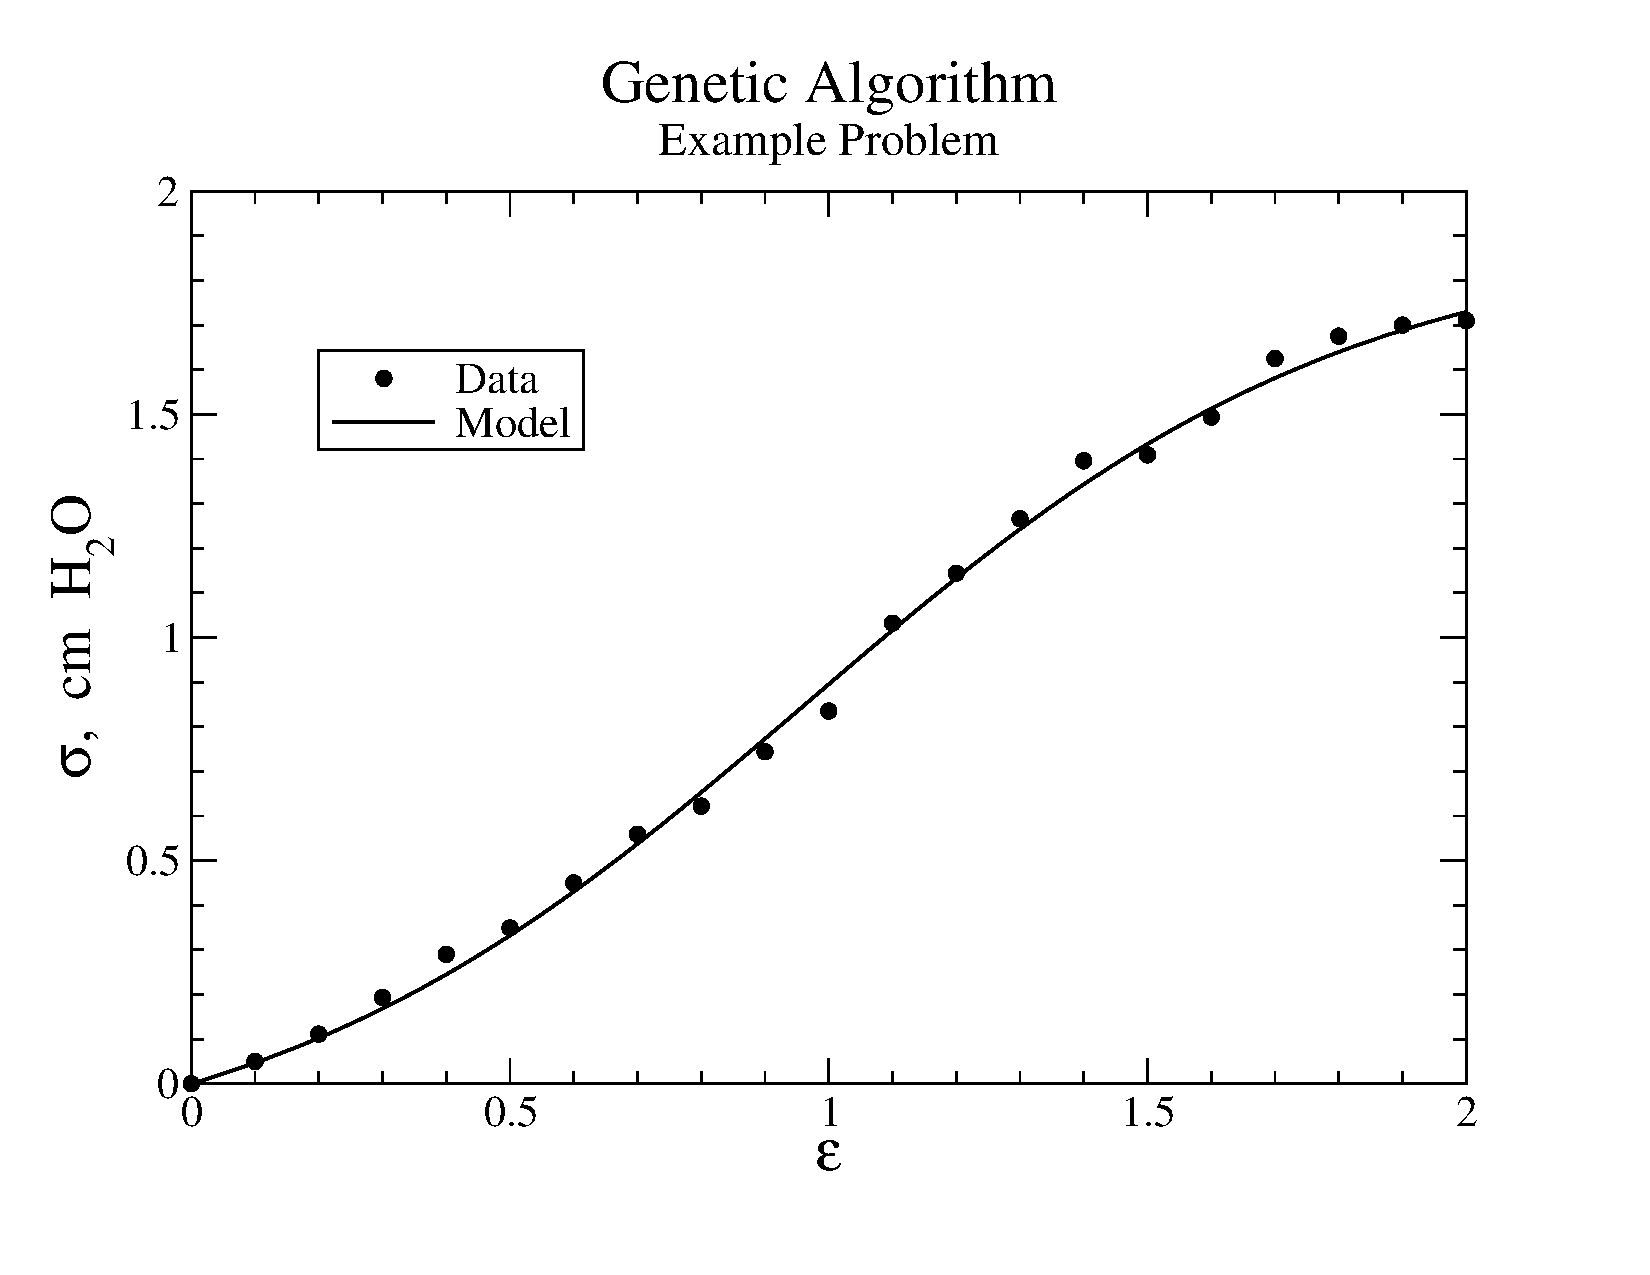
\includegraphics[height=6cm]{gaExample.pdf}
   \caption{GA fit to raw data, $\mathcal{R}^2 = 0.996$.}
   \label{exFigure}
\end{figure}

The example run of App.\ \ref{GaAppendix} required \scalar{19}
generations to reach theoretical convergence, given a population
size of \scalar{511}.  Values belonging to the most-fit creature
in the $i^{\text{th}}$ generation are reported; namely: the fitness
$\Phi_i$, the fraction of genes with the same allelic values
between the elite's parents, and the adjusted $\mathcal{R}^2_i$
statistic.  This is followed by a section that displays some of
the vital statistics of the run, \viz the numbers of crossovers,
mutations, and immigrants, the parameter estimates along with
measures of their sensitivity, and the \textsc{Gray} codes held
by the elite creature over the generations.

The `viable population size' of \scalar{4754} is the total
number of individuals over the whole history of the colony
whose parameters all fell within the sensitivity bounds
listed.  If one takes the population size, minus one for
the elite creature, and multiplies that by the number of
generations one arrives at the total number of creatures
over the history of the colony, adding 1 for the alien,
which in the case of this example was \scalar{9691}, as reported.
The average probability for crossover, for the whole colony,
is then $\mbox{\scalar{7942}} / \mbox{\scalar{9691}} = 0.8195$,
which lies between $P^c_{\text{max}} = 0.9$ and $P^c_{\text{min}}
= 0.6$, as expected.  Likewise, its average probability for mutation
is determined to be $\mbox{\scalar{8112}} / ( \mbox{\scalar{45}}
\times \mbox{\scalar{9691}}) = 0.0186$, which lies between
$P^m_{\text{max}} = 0.1$ and $P^m_{\text{min}} = 0.001$, again
as expected.

The time required to run this optimization problem was on
the order of a few seconds.


\section{History of Changes}
\fontsize{10pt}{12pt}\selectfont

\textsf{BEL} version releases wherein no change took place
in \textsf{BelGAlg} are omitted.  Version numbering corresponds 
with the version releases of \textsf{BEL}.


\subsection{Changes to Version 4.1}

Bug fixes.  Procedures \texttt{GeneticAlgorithm.Optimize} and 
\texttt{GeneticAlgorithm.EasyOptimize} are now functions.  
They return the optimal set of parameters found.  

\subsection{Changes to Version 4.0}

The concept of annealing was introduced via adaptive measures
for the probabilities of crossover and mutation.  The process
by which children are conceived was completely reworked, which
lead to simpler interface and usage of the optimizer.  A
capability to continue\slash stop an optimization run was added
to make the overall operation more user friendly.
Substantial changes to the interface resulted from fundamental
changes introduced through \texttt{Bel.Types}.


\subsection{Changes to Version 3.3}

The theoretical sections deriving the objective function,
the $\mathcal{R}^2$ statistic, and the sensitivity analysis
have been completely reworked.  The statistics are now a
tighter representation of what the author perceives as
being `reality'.  This major overhaul of module
\texttt{BelGAlg.Statistics} did somewhat affect its
interface, and consequently, the interfaces of modules
\texttt{Colonies} and \texttt{GeneticAlgorithm}, too.


\subsection{Changes to Version 3.0}

Removed \texttt{alienParameters} as an argument in procedure
\texttt{EasyOptimize}.


\subsection{Changes to Version 2.3}

A major internal change took place in that maximum likelihood
estimates, instead of maximum $R^2$ values, are now used as the
measure of fitness, i.e., the objective function.

Several bugs in \texttt{Bel.GA.Statistics} were fixed, including
an error in calculating the covariance matrix, and its interface,
\ie \texttt{Bel.GA.Statistics.Covariance}, was changed to make
the implementation more efficient.


\subsection{Changes to Version 2.1}

A bug was fixed that resulted from \textsf{BEL} GA being extracted from \textsf{BEL} to
become a standalone library.


\subsection{Changes to Version 2.0}

The genetic algorithm was extracted from the core \textsf{BEL} library as an
application library.


%\medskip\medskip
%\noindent{\large Acknowledgments}
%\medskip
%\noindent Add any if needed.

\bibliography{my}

\fontsize{12}{14.7}\selectfont

\onecolumn
\appendix

\section{Example GA Output}
\label{GaAppendix}

\begin{verbatim}
    --------------------------------------------------------------
    An optimization of 1 random variable over 20 events
                : --------------- most-fit citizen ---------------
    generation  :    fitness    : parent similarity : adjusted R^2
    --------------------------------------------------------------
         1        1.029834E+003      0.000E+000       9.89765E-001
         2        1.966732E+003      4.667E-001       9.85789E-001
         3        2.623127E+003      4.444E-001       9.93475E-001
         5        3.005862E+003      9.333E-001       9.96597E-001
         7        3.437132E+003      8.000E-001       9.96837E-001
        10        3.484098E+003      6.444E-001       9.96733E-001
        12        3.488700E+003      8.667E-001       9.96963E-001
        15        3.492407E+003      9.333E-001       9.96924E-001
        19        3.495432E+003      8.667E-001       9.96914E-001
    --------------------------------------------------------------
    total number of genes  = 45
    size of the population = 511
    number of contestants  = 10
    number of generations  = 19
    number of individuals  = 9691
    number of crossovers   = 7942
    number of mutations    = 8112
    number of immigrants   = 97
    --------------------------------------------------------------
    Optimum parameters, +/- 50% loss in significant-digit accuracy
    1)  1.071E+000 < 1.082E+000 < 1.093E+000
    2)  8.419E-001 < 8.504E-001 < 8.589E-001
    3)  4.505E-001 < 4.551E-001 < 4.596E-001
    Out of 9691 creatures, 4754 laid within these intervals.
    --------------------------------------------------------------
    gen : par)   -- genotype --
      1 :   1)   010010001101111
            2)   011001000101001
            3)   011111010101010
     ...
     10 :   1)   111010101000101
            2)   110011001001110
            3)   011000001100101
     ...
     19 :   1)   111010100100101
            2)   110011011010110
            3)   011000001001100
    --------------------------------------------------------------
\end{verbatim}

\section{Genetic Algorithm}
\label{gaAppendix}

The procedures inherited from the \textsl{[]}, \textsl{Bel.Entity},
\textsl{Bel.Object}, and \textsl{Bel.Typeset\/} definition interfaces
have been implemented in the actual code, but are not repeated here
to help keep the exported interfaces concise.

\medskip


\noindent\boldtt{module}\fonttt{ BelGAlg.Statistics;}

\indent\boldtt{import}

\indent\indent\fonttt{Bel.Types }\boldtt{as}\fonttt{ T;}


\indent\boldtt{var}\fonttt{ $\{$}\fontttsl{immutable}\fonttt{$\}$}

\indent\indent\fonttt{dimC, dimN, dimP, dimR\;:\;}\boldttsl{integer}\fonttt{;}


\indent\boldtt{type}

\indent\indent\fonttt{Model = }\boldtt{procedure}\fonttt{ (T.RealVector;
T.RealMatrix)\;:\;T.RealMatrix;}


\indent\boldtt{procedure}\fonttt{ FlipHeads (probabilityOfHeads\;:\;}\boldttsl{real}\fonttt{)\;:\;}\boldttsl{boolean}\fonttt{;}

\indent\boldtt{procedure}\fonttt{ RandomIntegerBetween (lowValue, highValue\;:\;}
\boldttsl{integer}\fonttt{)\;:\;}\boldttsl{integer}\fonttt{;}

\indent\boldtt{procedure}\fonttt{ Configure (expInput, expOutput\;:\;T.RealMatrix;}\\
\indent\indent\indent\indent\indent\indent\indent\indent\fonttt{decimateTo\;:\;}\boldttsl{integer}\fonttt{; numericalModel\;:\;Model;}\\
\indent\indent\indent\indent\indent\indent\indent\indent\fonttt{varyParameters\;:\;T.BooleanVector);}

\indent\boldtt{procedure}\fonttt{ DataFitAgainst (}\boldtt{var}\fonttt{ input, output\;:\;T.RealMatrix);}

\indent\boldtt{procedure}\fonttt{ Theory (parameters\;:\;T.RealVector)\;:\;T.RealMatrix;}

\indent\boldtt{procedure}\fonttt{ Fitness (parameters\;:\;T.RealVector)\;:\;}\boldttsl{real}\fonttt{;}

\indent\boldtt{procedure}\fonttt{ RSquared (parameters\;:\;T.RealVector)\;:\;}\boldttsl{real}\fonttt{;}

\noindent\boldtt{end}\fonttt{ Statistics.}



\medskip\medskip


\noindent\boldtt{module}\fonttt{ BelGAlg.Genes;}

\indent\boldtt{import}


\indent\indent\fonttt{Bel.Entity }\boldtt{as}\fonttt{ Entity,}

\indent\indent\fonttt{Bel.Typeset }\boldtt{as}\fonttt{ Typeset;}

\indent\boldtt{type}\fonttt{ Allele = }\boldttsl{integer}\fontttsl{$\{$8$\}$\/}\fonttt{;}

\indent\boldtt{type}\fonttt{ $\{$}\fontttsl{value}\fonttt{$\}$ Gene =
}\boldtt{object implements}\fonttt{ Entity, Typeset}

\indent\indent\boldtt{procedure}\fonttt{ Clone ()\;:\;Gene;}

\indent\indent\boldtt{procedure}\fonttt{ Pop ()\;:\;Allele;}

\indent\indent\boldtt{procedure}\fonttt{ Put (a\;:\;Allele);}

\indent\indent\boldtt{procedure}\fonttt{ Mutate (probabilityOfMutation\;:\;}\boldttsl{real}\fonttt{;}\\
\indent\indent\indent\indent\indent\indent\indent\indent\indent\boldtt{var}\fonttt{ numberOfMutations\;:\;}\boldttsl{integer}\fonttt{);}

\indent\indent\boldtt{procedure}\fonttt{ Equals (g\;:\;Gene)\;:\;}\boldttsl{boolean}\fonttt{;}

\indent\boldtt{end}\fonttt{ Gene;}

\indent\boldtt{operator ":="}\fonttt{ (}\boldtt{var}\fonttt{ l\;:\;Gene; r\;:\;Gene);}

\indent\boldtt{operator "="}\fonttt{ (l, r\;:\;Gene)\;:\;}\boldttsl{boolean}\fonttt{;}

\indent\boldtt{operator "\#"}\fonttt{ (l, r\;:\;Gene)\;:\;}\boldttsl{boolean}\fonttt{;}

\noindent\boldtt{end}\fonttt{ Genes.}


\medskip\medskip


\noindent\boldtt{module}\fonttt{ BelGAlg.Chromosomes;}

\indent\boldtt{import}

\indent\indent\fonttt{Bel.Entity }\boldtt{as}\fonttt{ Entity,}

\indent\indent\fonttt{Bel.Typeset }\boldtt{as}\fonttt{ Typeset,}

\indent\indent\fonttt{BelGAlg.Genes }\boldtt{as}\fonttt{ G;}

\indent\boldtt{type}\fonttt{ Haploid = }\boldtt{array * of}\fonttt{ G.Gene;}

\indent\boldtt{type}\fonttt{ $\{$}\fontttsl{ref}\fonttt{$\}$ Chromosome =
}\boldtt{object implements}\fonttt{ [], Entity, Typeset}

\indent\indent\boldtt{procedure}\fonttt{ Clone ()\;:\;Chromosome;}

\indent\indent\boldtt{procedure}\fonttt{ Create (minParameter, maxParameter\;:\;}\boldttsl{real}\fonttt{;}\\
\indent\indent\indent\indent\indent\indent\indent\indent\indent\fonttt{numberOfSignificantFigures\;:\;}\boldttsl{integer}\fonttt{);}

\indent\indent\boldtt{procedure}\fonttt{ Length ()\;:\;}\boldttsl{integer}\fonttt{;}

\indent\indent\boldtt{procedure}\fonttt{ Mutate (mutationProbability\;:\;}\boldttsl{real}\fonttt{;}\\
\indent\indent\indent\indent\indent\indent\indent\indent\indent\boldtt{var}\fonttt{ numberOfMutations\;:\;}\boldttsl{integer}\fonttt{);}

\indent\indent\boldtt{procedure}\fonttt{ Decode ()\;:\;}\boldttsl{real}\fonttt{;}

\indent\indent\boldtt{procedure}\fonttt{ Encode (phenotype\;:\;}\boldttsl{real}\fonttt{);}

\indent\indent\boldtt{procedure}\fonttt{ Equals (c\;:\;Chromosome)\;:\;}\boldttsl{boolean}\fonttt{;}

\indent\boldtt{end}\fonttt{ Chromosome;}

\indent\boldtt{operator "="}\fonttt{ (l, r\;:\;Chromosome)\;:\;}\boldttsl{boolean}\fonttt{;}

\indent\boldtt{operator "\#"}\fonttt{ (l, r\;:\;Chromosome)\;:\;}\boldttsl{boolean}\fonttt{;}

\indent\boldtt{procedure}\fonttt{ Crossover (probabilityOfCrossover\;:\;}\boldttsl{real}\fonttt{;}\\
\indent\indent\indent\indent\indent\indent\indent\indent\fonttt{parentA, parentB\;:\;Chromosome;}\\
\indent\indent\indent\indent\indent\indent\indent\indent\boldtt{var}\fonttt{
numberOfCrossovers\;:\;}\boldtt{integer}\fonttt{;}\\
\indent\indent\indent\indent\indent\indent\indent\indent\boldtt{var}\fonttt{ childA, childB\;:\;Chromosome);}

\noindent\boldtt{end}\fonttt{ Chromosomes.}



\medskip\medskip


\noindent\boldtt{module}\fonttt{ BelGAlg.Genomes;}

\indent\boldtt{import}

\indent\indent\fonttt{Bel.Entity }\boldtt{as}\fonttt{ Entity,}

\indent\indent\fonttt{Bel.Types }\boldtt{as}\fonttt{ T,}

\indent\indent\fonttt{BelGAlg.Chromosomes }\boldtt{as}\fonttt{ C;}

\indent\boldtt{type}\fonttt{ GenoType = }\boldtt{array * of}\fonttt{ C.Chromosome;}

\indent\boldtt{type}\fonttt{ $\{$}\fontttsl{ref}\fonttt{$\}$ Genome =
}\boldtt{object implements}\fonttt{ [], Entity}

\indent\indent\boldtt{procedure}\fonttt{ Clone ()\;:\;Genome;}

\indent\indent\boldtt{procedure}\fonttt{ Create (minParameters, maxParameters\;:\;T.RealVector;}\\
\indent\indent\indent\indent\indent\indent\indent\indent\indent\fonttt{numberOfSignificantFigures\;:\;}\boldttsl{integer}\fonttt{);}

\indent\indent\boldtt{procedure}\fonttt{ Equals (g\;:\;Genome)\;:\;}\boldttsl{boolean}\fonttt{;}

\indent\indent\boldtt{procedure}\fonttt{ Strands ()\;:\;}\boldttsl{integer}\fonttt{;}

\indent\indent\boldtt{procedure}\fonttt{ Mutate (probabilityOfMutation\;:\;}\boldttsl{real}\fonttt{;}\\
\indent\indent\indent\indent\indent\indent\indent\indent\indent\boldtt{var}\fonttt{ numberOfMutations\;:\;}\boldttsl{integer}\fonttt{);}

\indent\indent\boldtt{procedure}\fonttt{ Encode (phenotypes\;:\;T.RealVector);}

\indent\indent\boldtt{procedure}\fonttt{ Decode ()\;:\;T.RealVector;}

\indent\boldtt{end}\fonttt{ Genome;}

\indent\boldtt{operator "="}\fonttt{ (l, r\;:\;Genome)\;:\;}\boldttsl{boolean}\fonttt{;}

\indent\boldtt{operator "\#"}\fonttt{ (l, r\;:\;Genome)\;:\;}\boldttsl{boolean}\fonttt{;}

\indent\boldtt{procedure}\fonttt{ Crossover (probabilityOfCrossover\;:\;}\boldttsl{real}\fonttt{;}\\
\indent\indent\indent\indent\indent\indent\indent\indent\fonttt{parentA, parentB\;:\;Genome;}\\
\indent\indent\indent\indent\indent\indent\indent\indent\boldtt{var}\fonttt{ numberOfCrossovers\;:\;}\boldttsl{integer}\fonttt{;}\\
\indent\indent\indent\indent\indent\indent\indent\indent\boldtt{var}\fonttt{ childA, childB\;:\;Genome);}

\indent\boldtt{procedure}\fonttt{ Similarity (genomeA, genomeB\;:\;Genome)\;:\;}\boldttsl{real}\fonttt{;}

\noindent\boldtt{end}\fonttt{ Genomes.}


\medskip\medskip


\noindent\boldtt{module}\fonttt{ BelGAlg.Creatures;}

\indent\boldtt{import}

\indent\indent\fonttt{Bel.Entity }\boldtt{as}\fonttt{ Entity,}

\indent\indent\fonttt{Bel.Object }\boldtt{as}\fonttt{ Object,}

\indent\indent\fonttt{Bel.Types }\boldtt{as}\fonttt{ T,}

\indent\indent\fonttt{BelGAlg.Genomes }\boldtt{as}\fonttt{ G;}

\indent\boldtt{const}

\indent\indent\fonttt{minProbabilityOfMutation\;=\;0.001;}

\indent\indent\fonttt{maxProbabilityOfMutation\;=\;0.1;}

\indent\indent\fonttt{minProbabilityOfCrossover\;=\;0.6;}

\indent\indent\fonttt{maxProbabilityOfCrossover\;=\;0.9;}

\indent\boldtt{var}

\indent\indent\fonttt{birthNumber\;:\;}\boldttsl{integer}\fonttt{;}

\indent\boldtt{type}\fonttt{ $\{$}\fontttsl{ref}\fonttt{$\}$ Lineage =
}\boldtt{object implements }\fonttt{Object}

\indent\indent\boldtt{var}

\indent\indent\indent\fonttt{birthID\;:\;}\boldttsl{integer}\fonttt{;}

\indent\indent\indent\fonttt{fitness\;:\;}\boldttsl{real}\fonttt{;}

\indent\indent\indent\fonttt{parameters\;:\;T.RealVector;}

\indent\indent\indent\fonttt{parentSimilarity\;:\;}\boldttsl{real}\fonttt{;}

\indent\indent\indent\fonttt{probabilityOfMutation\;:\;}\boldttsl{real}\fonttt{;}

\indent\indent\indent\fonttt{probabilityOfCrossover\;:\;}\boldttsl{real}\fonttt{;}

\indent\boldtt{end}\fonttt{ Lineage;}

\indent\boldtt{type}\fonttt{ $\{$}\fontttsl{ref}\fonttt{$\}$ Creature =
}\boldtt{object implements}\fonttt{ Entity}

\indent\indent\boldtt{var}\fonttt{ $\{$}\fontttsl{immutable}\fonttt{$\}$}

\indent\indent\indent\fonttt{lineage\;:\;Lineage;}

\indent\indent\boldtt{procedure}\fonttt{ Clone ()\;:\;Creature;}

\indent\indent\boldtt{procedure}\fonttt{ Create (fixedParameters\;:\;T.RealVector;}\\
\indent\indent\indent\indent\indent\indent\indent\indent\indent\fonttt{varyParameters\;:\;T.BooleanVector);}

\indent\indent\boldtt{procedure}\fonttt{ Get ()\;:\;G.Genome;}

\indent\indent\boldtt{procedure}\fonttt{ Alien (parameters, minParameters, maxParameters\;:\;T.RealVector;}\\
\indent\indent\indent\indent\indent\indent\indent\indent\indent\fonttt{numberOfSignificantFigures\;:\;}\boldttsl{integer}\fonttt{);}

\indent\indent\boldtt{procedure}\fonttt{ Procreate (minParameters, maxParameters\;:\;T.RealVector;}\\
\indent\indent\indent\indent\indent\indent\indent\indent\indent\fonttt{numberOfSignificantFigures\;:\;}\boldttsl{integer}\fonttt{;)}

\indent\indent\boldtt{procedure}\fonttt{ Conceive (parentA, parentB\;:\;Creature;}\\
\indent\indent\indent\indent\indent\indent\indent\indent\indent\boldtt{var}\fonttt{ numberOfMutations, numberOfCrossovers\;:\;}\boldttsl{integer}\fonttt{);}

\indent\indent\boldtt{procedure}\fonttt{ Equals (c\;:\;Creature)\;:\;}\boldttsl{boolean}\fonttt{;}

\indent\indent\boldtt{procedure}\fonttt{ AssignProbabilities (maxFitness, avgFitness\;:\;}\boldttsl{real}\fonttt{);}

\indent\boldtt{end}\fonttt{ Creature;}

\indent\boldtt{operator "="}\fonttt{ (l, r\;:\;Creature)\;:\;}\boldttsl{boolean}\fonttt{;}

\indent\boldtt{operator "\#"}\fonttt{ (l, r\;:\;Creature)\;:\;}\boldttsl{boolean}\fonttt{;}

\noindent\boldtt{end}\fonttt{ Creatures.}



\medskip\medskip


\noindent\boldtt{module}\fonttt{ BelGAlg.Colonies;}

\indent\boldtt{import}

\indent\indent\fonttt{System.IO.StreamWriter }\boldtt{as}\fonttt{ StreamWriter,}

\indent\indent\fonttt{Bel.Entity }\boldtt{as}\fonttt{ Entity,}

\indent\indent\fonttt{Bel.Types }\boldtt{as}\fonttt{ T,}

\indent\indent\fonttt{BelGAlg.Statistics }\boldtt{as}\fonttt{ S,}

\indent\indent\fonttt{BelGAlg.Creatures }\boldtt{as}\fonttt{ C;}

\indent\boldtt{type}\fonttt{ Inhabitants = }\boldtt{array * of}\fonttt{ C.Creatures;}

\indent\boldtt{type}\fonttt{ $\{$}\fontttsl{ref}\fonttt{$\}$ Colony =
}\boldtt{object implements}\fonttt{ Entity}

\indent\indent\boldtt{procedure}\fonttt{ Create (expInput, expOutput\;:\;T.RealMatrix;}\\
\indent\indent\indent\indent\indent\indent\indent\indent\fonttt{decimateTo\;:\;}\boldttsl{integer}\fonttt{; numericalModel\;:\;S.Model;}\\
\indent\indent\indent\indent\indent\indent\indent\indent\fonttt{varyParameters\;:\;T.BooleanVector;}\\
\indent\indent\indent\indent\indent\indent\indent\indent\fonttt{fixedParameters, alienParameters,}\\
\indent\indent\indent\indent\indent\indent\indent\indent\fonttt{minParameters, maxParameters\;:\;T.RealVector;}\\
\indent\indent\indent\indent\indent\indent\indent\indent\fonttt{dimensionOfSchemata,}\\
\indent\indent\indent\indent\indent\indent\indent\indent\fonttt{numberOfSignificantFigures\;:\;}\boldttsl{integer}\fonttt{);}

\indent\indent\boldtt{procedure}\fonttt{ Propagate (}\boldtt{var}\fonttt{ converged\;:\;}\boldttsl{boolean}\fonttt{);}

\indent\indent\boldtt{procedure}\fonttt{ Parameters ()\;:\;T.RealVector;}

\indent\indent\boldtt{procedure}\fonttt{ ReportHeader (sw\;:\;StreamWriter);}

\indent\indent\boldtt{procedure}\fonttt{ ReportBody (sw\;:\;StreamWriter);}

\indent\indent\boldtt{procedure}\fonttt{ ReportFooter (sw\;:\;StreamWriter);}

\indent\indent\boldtt{procedure}\fonttt{ CheckOnTheState (}\boldtt{var}\fonttt{
finished\;:\;}\boldttsl{boolean}\fonttt{);}

\indent\boldtt{end}\fonttt{ Colony;}

\noindent\boldtt{end}\fonttt{ Colonies.}


\medskip\medskip


\noindent\boldtt{module}\fonttt{ BelGAlg.GeneticAlgorithm;}

\indent\boldtt{import}

\indent\indent\fonttt{Bel.Types }\boldtt{as}\fonttt{ T,}

\indent\indent\fonttt{BelGAlg.Statistics }\boldtt{as}\fonttt{ S;}

\indent\boldtt{procedure}\fonttt{ Optimize (fileNameForReport\;:\;}\boldttsl{string}\fonttt{;}\\
\indent\indent\indent\indent\indent\indent\indent\indent\fonttt{expInput, expOutput\;:\;T.RealMatrix;}\\
\indent\indent\indent\indent\indent\indent\indent\indent\fonttt{decimateTo\;:\;}\boldttsl{integer}\fonttt{; numericalModel:\;S.Model;}\\
\indent\indent\indent\indent\indent\indent\indent\indent\fonttt{varyParameters\;:\;T.BooleanVector;}\\
\indent\indent\indent\indent\indent\indent\indent\indent\fonttt{fixedParameters, alienParameters,}\\
\indent\indent\indent\indent\indent\indent\indent\indent\fonttt{minParameters, maxParameters\;:\;T.RealVector;}\\
\indent\indent\indent\indent\indent\indent\indent\indent\fonttt{dimensionOfSchemata,}\\
\indent\indent\indent\indent\indent\indent\indent\indent\fonttt{numberOfSignificantFigures\;:\;}\boldttsl{integer}\fonttt{)}\\
\indent\indent\indent\indent\indent\indent\indent\indent\fonttt{:\;T.RealVector;}

\indent\boldtt{procedure}\fonttt{ EasyOptimize (fileNameForReport\;:\;}\boldttsl{string}\fonttt{;}\\
\indent\indent\indent\indent\indent\indent\indent\indent\fonttt{expInput, expOutput\;:\;T.RealMatrix;}\\
\indent\indent\indent\indent\indent\indent\indent\indent\fonttt{numericalModel\;:\;S.Model;}\\
\indent\indent\indent\indent\indent\indent\indent\indent\fonttt{minParameters, maxParameters\;:\;T.RealVector)}\\
\indent\indent\indent\indent\indent\indent\indent\indent\fonttt{:\;T.RealVector;}

\noindent\boldtt{end}\fonttt{ GeneticAlgorithm.}


\end{document}
